
\documentclass[letterpaper]{article}
%\usepackage[utf8]{inputenc}
\usepackage[inner=4.67cm, outer=3.33cm, top=2.54cm, bottom=3cm]{geometry} 
\usepackage[english]{babel}
\usepackage[autostyle]{csquotes}
\usepackage{svg}
\usepackage{amsmath} % provides miscellaneous enhancements for improving the information structure and printed output of documents containing mathematical formulas 
\usepackage{amsfonts,amssymb} % amssymb provides an extended symbol collection and internally loads amsfonts Computer Modern font plus a set of miscellaneous TeX fonts that augment the standard Computer Modern set
\usepackage{hyperref}
\hypersetup{
    colorlinks=true,
    linkcolor=blue,
    filecolor=magenta,      
    urlcolor=cyan,
    pdftitle={Overleaf Example},
    pdfpagemode=FullScreen,
    }
\usepackage{graphicx} % show images
\usepackage{multirow} % for multirow in tables
\usepackage{hhline} % for double lines without interrupting table vertical lines
\usepackage{array}
\graphicspath{ {images/} } % Path relative to the .tex file containing the \includegraphics command
\usepackage{siunitx} % comprehensive (si) units package and overleaf chokes on [=v3]
% begin itemize and enumerate formatting
\usepackage{enumitem} % Control layout of itemize, enumerate, description
\setlist{nolistsep} % removes space between list and enumerate items
% end itemize and enumerate formatting
\usepackage[skip=0.5\baselineskip]{caption} % allows addition of space after the caption and prior to the table
\usepackage{tikz,lmodern}
\usepackage[most]{tcolorbox}

%================================================
% begin paragraph formatting if no first line indent and space between
% \usepackage{parskip} % adds space between paragraphs
% \setlength{\parindent}{0pt} % Default is 15pt thus no first line indent
\setlength{\parindent}{15pt} % Set to 0pt for no first line indent
%\setlength{\parskip}{2mm plus1mm minus1mm} % adds space between paragraphs
% \setlength{\parskip}{\baselineskip} % adjusts added space between paragraphs
% end paragraph formatting
%==================================================

%==========================================================
% Attribution — You must give appropriate credit, provide a link to the
%   license, and indicate if changes were made. You may do so in any
%   reasonable manner, but not in any way that suggests the licensor endorses
%   you or your use.
% ShareAlike — If you remix, transform, or build upon the material, you must
%   distribute your contributions under the same license as the original.
%==========================================================
% The greater community benefits if any corrections or additions as changes made to this source are offset in the code with contributors contact information.
%==========================================================
%+Title
  \title{\Huge\bf\ Soil Physical Properties\\ \, \\\normalsize Version: Beta 0.7}
  \author{Donald G. McGahan\\}
  \date{August 3, 2022}
%-Title
\begin{document}
\maketitle
\section*{Copyright}

The Soil Physical Properties by Donald G. McGahan is licensed under a \href{https://creativecommons.org/licenses/by-sa/4.0/}{Creative Commons Attribution-ShareAlike 4.0 International (CC BY-SA 4.0)} 

\par{\centering
\includegraphics[width=0.2\textwidth]{images/by-sa.png}\par} %centers graphic

\section*{Source code}

The LaTeX source code is at \href{https://github.com/dig-soilman/Soil_Physical_Properties.git}{https://github.com/dig-soilman/Soil\_Physical\_Properties.git}.

%
%\tableofcontents
%\listoffigures
%\listoftables

\section{Introduction}
\label{introduction}

Descriptions of the physical properties of soil include size separates, organization of size separates, density, voids or porosity, color, reaction, effervescence and consistence. These are properties that can be seen, felt, and tasted.

Initial recordings of physical properties are to be just that, an assessment of the observation and a recording. But record what? Each property has been assigned a sensible scaler. Frequently, the method to determine what is recorded can sometimes be an actual measurement but can be that of a categorical class agreed upon by users at large. Different groups may leverage different categorical classes. 

In this introductory treatise of soil physical properties, examples of categorizing the information is presented. The categorical classes presented are those used in practice by the United Stated Department of Agriculture (USDA) Soil Survey Division Staff when describing soil.

Many of the physical descriptions may be performed where the soil lives. A few determinations are routinely finished off site. Oven drying clods to determine the soils bulk density is notable here. Another is that although the soils apparent texture is generally determined at the excavation it is routine to also accomplish a laboratory determination of the soil basic textural class.

These classes of each categorical overlay are part of the data that is collated and parsed to place soil into a natural classification called \textbf{Soil Taxonomy}. Other uses of the presented classes are technical classification systems as opposed to the natural classification system of Soil Taxonomy. Therefore, the underlying measurements introduced in this treatment and the organizing of the measurements into classes represent the data that is used to convey information about how the soil exists and how it might be leveraged for a plethora of uses.

Below, each of the properties introduced might easily be expanded upon in a more complete treatise of their own. The goal of this treatise is to present each property in a manner that introduces each subtopic and presents some utilization of each subtopic in preparation for further study and use of information about soils.

%=========================================================================
% \section{Objectives}
% \label{objectives}

% TODO dig-soilman: populate an objectives section. 

% Present and define the USDA particle size separates classes.
% Present methods to determine particle size separates class.
%---------------------------------
% Explain how to determine one of the USDA twelve basic textural classes.
% TODO dig-soilman: A better dialog can be presented to achieve this objective
%   with respect to pipette and hydrometer method and can borrow from Soil
%   Laboratory Exercise Manual
%----------------------------------
% Present how coarse fraction modifiers are applied to USDA twelve basic
%   textural classes.
% Define soil bulk density.
% Present how to calculate soil bulk density.
% Define soil porosity.
% Present how to calculate soil porosity.
% Define soil structure and the soil structure types.
% Introduce soil structure sizes and grades.
% Relate void size to soil texture and structure.
% Introduce available water retention and movement to void size and structure.
%------------------------------------
% Describe how soil color is recorded and its inference to reduction and oxidation which is tied to water and air and biologicals.
% TODO dig-soilman: a very brief introduction that biologicals drive reduction and thereby the colors and patterns from mobility of elements like iron. This would me more fully elucidated in a treatise of Soil Chemistry.
%-------------------------------
% Introduce reactivity (pH) classes.
%   Reactivity would be more fully expanded in a treatise of Soil Chemistry.
%-----------------------------------
% Introduce effervescence classes.
% TODO dig-soilman: Effervescence needs a little more attention but would be more fully explored in a Soil Water Chapter (Could call a treatise with suggested title Soil Climate and do temperature in the same chapter with water.)
%=========================================================================

\section{Organic Soil}
\label{organic_soil}
    
Soil solids can be mineral or organic in nature. A soil that consists of primarily accumulated plant material of various degrees of decomposition are separated from soils derived from dominantly mineral materials. The use of the term \textbf{organic soil} in this treatise is that defined by the U.S. Department of Agriculture. To be considered an organic soil:
    
\begin{enumerate}
    \item Soil that is never saturated with water for more than a few days must contain more than \qty{20}{\percent} organic carbon.
    \item If the soil is saturated for periods longer than a few days, it is organic if it contains the following:
    \begin{itemize}
        \item At least \qty{12}{\percent} organic carbon if the soil has not clay,
        \item At least \qty{18}{\percent} percent organic carbon if the soil has 60 percent or more clay, or 
        \item If it contains a proportional amount of organic carbon for intermediate amounts of clay.
    \end{itemize}
\end{enumerate}
    
The percentages are determined on a mass basis. A conversion factor of \num{1.72} is commonly used to convert organic carbon to organic matter. This conversion factor assumes organic matter contains \qty{58}{\percent} organic carbon. However this can vary with the type of organic matter, soil type and soil depth. Conversion factors can be as high as \num{2.50}, especially for subsoils.

Today it is common to determine soil organic carbon by an laboratory ignition method consisting of placing a known mass of soil in a furnace and quantifying the carbon released as a gas. Soil can also contain inorganic carbon. Quantification of organic carbon begins at the excavation by describing the effervescence class Table \ref{tab:effervescenceclasses}. Other wet chemistry techniques exist but are largely supplanted by the total carbon method by ignition. 

Most soils have some organic carbon but are below the levels necessary to attain the organic soil name. The inorganic or mineral fraction of the soil are measured and classified based on size.
    
\section{Classifying Mineral Size Separates}
    
Separates are the individual particles that together with organics, salts, and evaporates comprise a soil. We size them by placing them together in groupings that have a range in size with an upper and lower effective spherical diameter. The choice for the range in size is dictated by properties that one ‘size range’ exhibits, that is different than other size ranges. Often these can be grouped for particular purposes. The groupings once formalized are termed ‘classes.’ The term fraction is used to connote part of a whole.

It is noteworthy to state that n=mineral size separates are  based on only the mineral fraction. Organics, salts, and evaporites are not included as part of the whole in determination and reporting.

We initially group the separates of the “whole” of the mineral  soil into two classes, the coarse fraction (CF) and the fine-earth fraction. The coarse fraction consists of the particles greater than \qty{2}{mm} in diameter and the fine-earth fraction consist of particles equal to and less than \qty{2}{mm}.

Both the coarse fraction and fine-earth fraction are further divided, again, on the basis of size. The fine-earth fraction is divided first into three size separates: sand, silt, and clay.

\begin{tcolorbox}[enhanced, attach boxed title to top center={yshift=-3mm, yshifttext=-1mm}, colback=yellow!18!white, colframe=red!55!black, colbacktitle=red!65!black, title=USDA Groupings and Subgroupings,fonttitle=\bfseries, boxed title style={size=small,colframe=red!50!black} ]
     \textbf{Coarse Fraction} are separates greater in diameter than \qty{2}{mm}.
    
    \textbf{Fine-Earth Fraction} are separates less than or equal to \qty{2}{mm}.
\end{tcolorbox}

    
Coarse fragments, or the coarse fraction, are important to consider because they occupy space in the soil, but contribute little or no voids (water and air storage) and chemical reactivity (nutrient storage). Thus, coarse fragments reduce the soil volume available to hold water and nutrients. Coarse fragments may also make cultivation difficult.

\subsection{Particle Size} \label{particlesize}
    
Soil texture refers to the proportion groupings of size separates in the inorganic soil fine earth fraction (\qty{< 2}{mm} in diameter). There are generally three groupings with further divisions of the three to achieve more refined interpretive relevance. The three groupings of the fine earth fraction are sand, silt, and clay.
    
The sands are the separates between \qtyrange{0.05}{2}{mm}.

The sand size separates are further classed into five size classes. The sand is further divided. \textit{Very Coarse Sand} separates are from \qtyrange{2}{1}{mm} diameter. \textit{Coarse Sand} separates are from \qtyrange{1}{0.5}{mm} diameter. \textit{Medium Sand} separates are from \qtyrange{0.5}{0.25}{mm} diameter. \textit{Fine Sand} separates are from \qtyrange{0.25}{0.10}{mm} diameter. \textit{Very Fine Sand} separates are from \qtyrange{0.10}{0.05}{mm} diameter.

Silt are separates are between the diameters of \qtyrange{0.002}{0.05}{mm} or \qtyrange{2}{50}{\micro\metre} where \qty{1000}{\micro\meter} are in \qty{1}{\milli\meter}.

Clay are separates with diameters of \qty{ \leq 0.002}{mm} or \qty{2}{\micro\metre}.

\subsection{Textural Triangle}
    
A Gibbs triangle, commonly referred to as a textural triangle, is a ternary diagram that relates the relationship between the sand, silt, and clay mass proportions and helps place the relationship of these size separates into a \textbf{Textural Class}. There are twelve basic soil textural classes in the system is presented in Figure \ref{fig:TexturalTriangle}.

Sand, Loamy Sand, Sandy Loam, Sandy Clay Loam, Silt, Silt Loam, Silty Clay Loam, Loam, Clay Loam, Clay, Silty Clay, and Sandy Clay.

It is important to note that the sand, silt, and clay mass proportions represented as a percent of the fine earth fraction add up to 100 percent. Organic matter and coarse fraction is not included when determining the textural class.

Texture can generally not be readily changed, except at great expense (example: adding sand to your garden).

\begin{center}
Sand\% + Silt\% + Clay\% = 100\%
\end{center}
    
\begin{figure*}
    \centering
    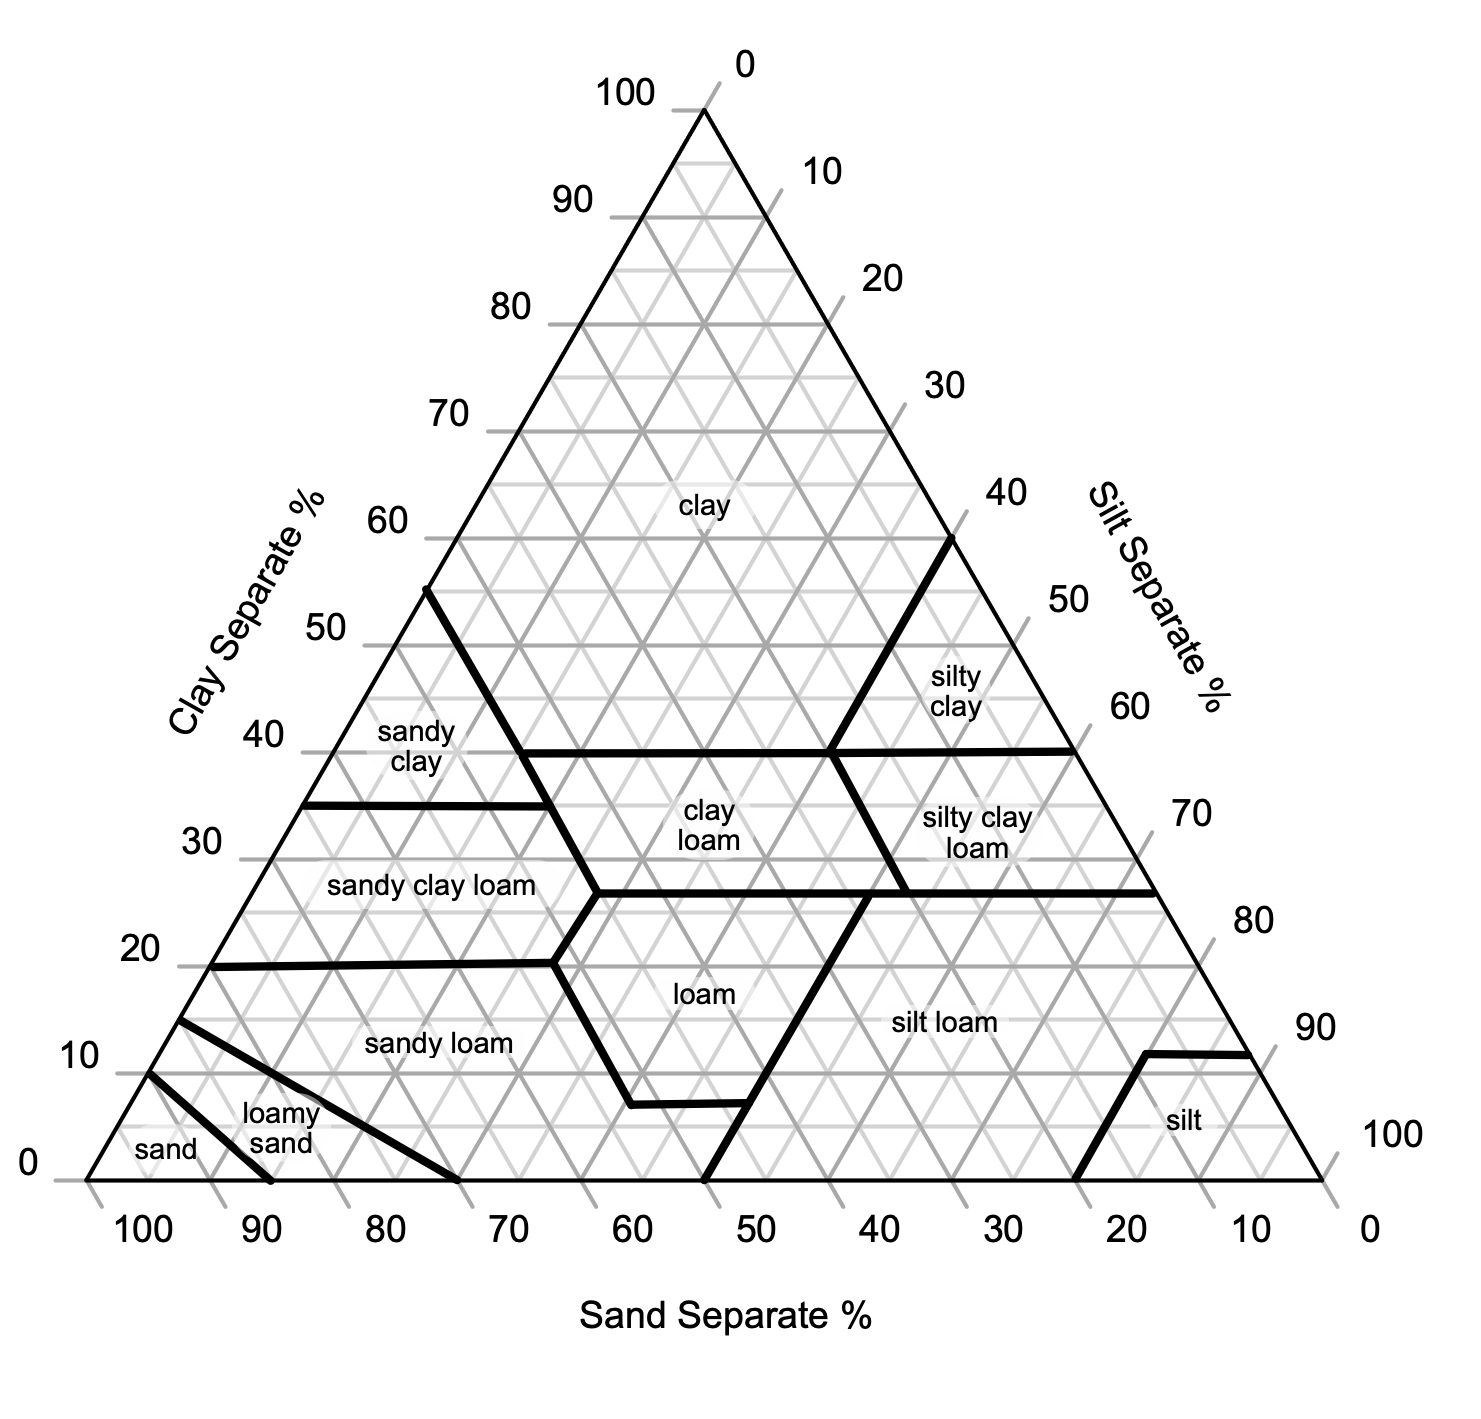
\includegraphics[width=0.98\columnwidth]{images/Textural_Triangle-wo-background.png}
    \caption{Gibbs Triangle or commonly called a Textural Triangle depicting the twelve basic textural classes of the USDA system as determined by the mass percentage of clay, silt, and sand size separates. Figure: Donald G. McGahan Creative Commons Attribution-ShareAlike-4.0-International.}
    \label{fig:TexturalTriangle}
\end{figure*}

 \begin{tcolorbox}[enhanced, attach boxed title to top
 	center={yshift=-3mm, yshifttext=-1mm}, colback=yellow!18!white, colframe=red!55!black, colbacktitle=red!65!black, title=USDA 12 basic textural classes, fonttitle=\bfseries,
  boxed title style={size=small, colframe=red!50!black} ]
     Sand, Loamy Sand\\
     Sandy Loam\\
     Loam, Silt Loam, Silt\\
     Clay Loam, Sandy Clay Loam, Silty Clay Loam\\ 
     Clay, Sandy Clay, Silty Clay
\end{tcolorbox}
    
Loam is a soil textural class in which the sand, silt and clay fractions have a similar influence on soil properties, but are not in equal proportions.

Some of the textural classes can be further subdivided. Such a refinement is usually based upon sand distribution e.g. Loamy \textbf{Very Fine} Sand.

Each of these twelve textural class names may have a coarse fraction modifier added when the coarse fraction exceeds 15\% of the soil horizons volume. Note that the assignment to one of the textural classes on a mass basis but the coarse fraction contribution is determined on a volume basis.

The coarse Fraction is divided into four (4) classes: \textit{gravel}, \textit{cobble}, \textit{stone}, and \textit{boulder} (Table \ref{tab:coarsefractionsizenames}).

The implications of coarse fraction is that the coarse fraction does not participate in water retention and can have an impact on tillage operations.

If two or more coarse fraction sizes exist, the entire volume of the coarse fraction is used for the modifier.

The largest size fraction is named, unless a smaller fraction is more than twice the volume of the larger size fraction and then that smaller fraction modifier is used as the modifier.
    
\subsection{Determination of soil texture}

The field method of determining textural class is the \enquote{feel method} where sand feels gritty, silt feels smooth or floury, and clay feels sticky. The subsequently determined proportions are classed as an \enquote{apparent texture}.

Professional practitioners aim to determine the apparent textural class of the twelve category textural class system. Figure \ref{fig:TextureByFeelFlowChart12} provides a decision tree to guide the determination.

\begin{figure*}
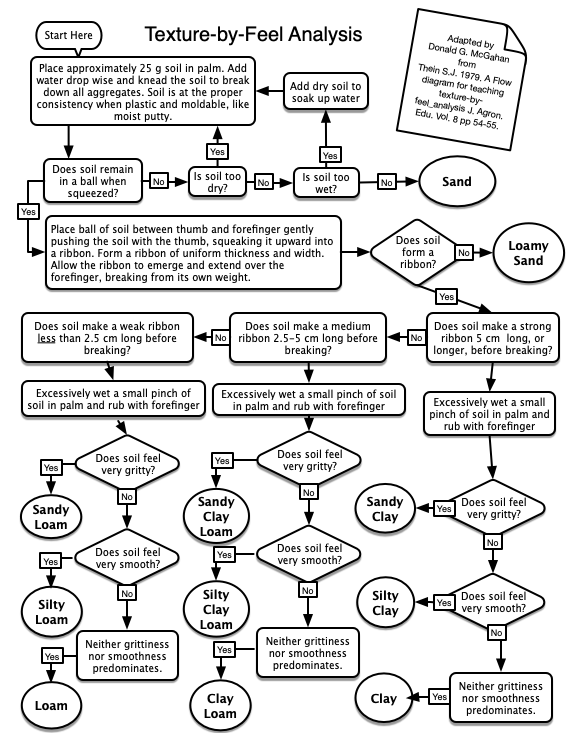
\includegraphics[width=0.98\columnwidth]{images/Texture_by_feel_analysis_DecissionTree-12-Category-bw-72pxpin-576x733px.png}
\caption{Texture-by-Feel Analysis decision flow chart to determine one of eleven of the twelve basic textural classes. The resulting determination of a textural class would be said to be an "apparent texture". Note that Silt is the basic textural class not on the decision flow chart. Figure: Donald G. McGahan Creative Commons Attribution-ShareAlike-4.0-International.} 
\label{fig:TextureByFeelFlowChart12}
\end{figure*}
% the above adaption figure has been adapted by others e.g. USDA-NRCS \href{https://www.nrcs.usda.gov/wps/portal/nrcs/detail/soils/edu/?cid=nrcs142p2_054311}{https://www.nrcs.usda.gov/wps/portal/nrcs/detail/soils/edu/?cid=nrcs142p2_054311} NOT SURE ABOUT attaining permissions.

\subsubsection{Laboratory Determination of Size Separates}

Laboratory procedures to determine the actual textural class begins by separation of the coarse fraction from the fine earth fraction via a 2-mm sieve. The coarse fraction volume is determined utilizing Archimedes principle of liquid displacement. The coarse fraction is reported as volume whereas the fine earth fractions are reported as mass.

Pretreatments to the 2~mm and smaller mineral fraction enhance separation of the size separates. Coarser organic matter is removed and the humus fraction of organic matter is oxidized with hydrogen peroxide. Salts can be removed by passing water through the soil. Carbonates can be evolved with a weak acid such as glacial acetic acid and mild heat. Iron can be reduced and chelated for removal.

The remaining \qty{2}{mm} and smaller mineral fraction separates are then dispersed with sodium hexametaphosphate with mixing, and the \qtyrange{2000}{50}{\micro\metre} sands are separated by sieving from the $\leq$ \qty{50}{\micro\metre} separates silt fraction and clay fraction. Sampling an aliquot of the suspension at a specified depth via a pipette to isolate the $\leq$ \qty{2}{\micro\metre} clay follows dispersion and sedimentation.

Such pipette sampling is considered to be the “platinum standard” for textural analysis.

Sampling time for the plane above where the silt fraction has passed below is determined via a modified form of Stokes’ Law for sedimenting soil suspensions:

\noindent\begin{minipage}{\textwidth}
\begin{equation}
    t=\frac{18\eta h}{[g\,(\rho_s - \rho_l)d^2]}
\end{equation}
\begin{equation*}
    \begin{aligned}
        \text{where}                                          \\
        t &= \text{time}                                      \\
        \eta &= \text{fluid viscosity}                        \\
        h &= \text{-height above plane z; the sampling depth} \\
        d &= \text{diameter of the separate}                  \\
        g &= \text{acceleration due to gravity}               \\
        \rho_s &= \text{particle density solid}               \\
        \rho_l &= \text{liquid density}
    \end{aligned}
\end{equation*}
\end{minipage}
        
Frequently the density of the size separates are assumed and the particles are assumed to be spherical.

% ToDo dig-soilman: add citation in references for Bouyoucos.

Bouyoucos devised a hydrometer method in an effort to simplify the measurement of sand, silt, and clay for a given soil. The initial methodology required two readings. The initial reading at 40 seconds to differentiate between the mass of soil without sand proves to be quite inaccurate. The modified Bouyoucos forgoes the 40 second reading and calls for sieving the sand out of the suspension. This negates much of the time savings of the original method. Additionally, with textural classes sand, sandy loam, and loamy sand the sand might need to be fractionated anyway for proper subclass modification of the sand. Thus, sieving to retain the sand can have practical benefits.

The sand is further fractionated via dry sieving. The amount of each of the sand sub-fractions becomes important for soils with textural class of sand, loamy sand, or sandy loam soils wherein the sand might earn a \textit{coarse}, \textit{fine} or \textit{very fine} modifier. See Soil Survey Manual 2017 for more on sand textures subclasses.

Note that the silt fraction is further separated into fine and coarse. The silt size has particular importance to the mechanical properties of the silt size and is useful for classing for erosion.

In an introductory soils coarse students are responsible for the size limits of the coarse fraction and fine earth fraction. Within the fine earth fraction introductory soils coarse students are responsible for the size limits of clay, silt, and sand (Section \ref{particlesize}). 

As presented in the particle size subsection sands are also subdivided. Memorizing the sand fractions (Table \ref{tab:sandfractions}) is particularly useful since these sizes often show up in names of soil map units. Soil map units convey information about patterns of spatial variability across the landscape.

\begin{table}[!htbp]
\centering
\caption{Table of sand fraction names and size limits.}
\label{tab:sandfractions}
\begin{tabular}{|lc|}
\hline
Sand Separate    & Diameter (mm) \\ \hhline{|==|}
very fine sand   & 0.05 – 0.10   \\
fine sand        & 0.10 – 0.25   \\
medium sand      & 0.25 – 0.50   \\
coarse sand      & 0.50 – 1.00   \\
very coarse sand & 1.00 – 2.00   \\
\hline
\end{tabular}
\end{table}

% dig-soilman: Markdown table rendering below of the above LaTeX table.
% Table of coarse fraction (CF) content volume percentage and modifier names.
% | Sand Separate    | Diameter (mm) |
% |:-----------------|:-------------:|
% | very fine sand   | 0.05 – 0.10   |
% | fine sand        | 0.10 – 0.25   |
% | medium sand      | 0.25 – 0.50   |
% | coarse sand      | 0.50 – 1.00   |
% | very coarse sand | 1.00 – 2.00   |

\begin{table}[!htbp]
\centering
\caption{Table of coarse fraction (CF) content volume percentage 
    and modifier names.}
\label{tab:coarsefractionvolume}
\begin{tabular}{|ll|}
\hline
\% Volume of CF  &  Modifier Name                        \\  \hhline{|==|}
0-15             & no modifier                           \\
15-35            & gravelly, cobbly, stony, or bouldery  \\
35-60            & add very e.g. very gravelly           \\
\textgreater{}60 & add extremely e.g. extremely gravelly \\
\hline
\end{tabular}
\end{table}

% dig-soilman: Markdown table rendering below of the above LaTeX table.
% Table of coarse fraction (CF) content volume percentage and modifier names.
% | % Volume of CF | Modifier Name                          |
% |:---------------|:---------------------------------------|
% | 0-15           | no modifier                            |
% | 15-35          | gravelly, cobbly, stony, or bouldery   |
% | > 60           | add extremely e.g. extremely gravelly  |

\begin{table}[!htbp]
\centering
\caption{Table of coarse fraction separates size increments.}
\label{tab:coarsefractionsizenames}
\begin{tabular}{|l c|}
\hline
Name        &  Size                \\ \hhline{|==|}
Gravel      & 2-75 mm              \\
Cobble      & 75-250 mm            \\
Stone       & 250-600 mm           \\
Boulder     & \textgreater{}600 mm \\
\hline
\end{tabular}
\end{table}

% dig-soilman: Markdown table rendering below of the above LaTeX table.
% Table of coarse fraction separates size increments.
% |   Name  | Size       |
% |:--------|:----------:|
% | Gravel  | 2-75 mm    |
% | Cobble  | 75-250 mm  |
% | Stone   | 250-600 mm |
% | Boulder | > 600 mm   |

% start box to offset more advanced "introduce only" item meant to be address in a separate treatise perhaps labeled "Classification"
\begin{center}
\fbox{\fbox{\parbox{5.0in}{
In more advanced courses students are likely asked to be responsible for the size limits of the fine silt and coarse silt, and occasionally even the clay which is fractionated into:
    
\begin{itemize}
    \item fine clay \qty{< 0.00008}{mm}, or \qty{< 0.08}{\micro\meter}
    \item medium clay \qtyrange{0.00008}{0.0002}{mm}, or \qtyrange{0.08}{0.2}{\micro\meter}
    \item coarse clay \qtyrange{0.0002}{0.002}{mm}, or \qtyrange{0.2}{2}{\micro\meter}
\end{itemize}
    
The amount of fine clay is particularly important when classifying some soils in Soil Taxonomy.}}}
\end{center}
% end box to offset more advanced introduce only item      


\subsubsection{Texture Grouping}

It is common, frequent, and convenient to speak more broadly, generally, or more inclusively about classes of soil texture. Commonly employed is referring to soil materials as \textit{General texture groupings} of \textbf{sandy}, \textbf{loamy}, or \textbf{clayey}. When the three General texture grouping terms are used in discussion it is helpful to think about the way in which these three terms are used to guide if the term is a General texture grouping or a textural category from the twelve basic textural classes. This can initially be confusing to the uninitiated so when it doubt, ask, because a \textit{sandy, loamy, or clayey} soil materials reference–general textural grouping terms–is not the same as \textit{sand, loam, or clay} textural class terms from the twelve basic textural classes.

\begin{tcolorbox}[enhanced, attach boxed title to top center={yshift=-3mm, yshifttext=-1mm}, colback=yellow!18!white, colframe=red!55!black, colbacktitle=red!65!black, title=USDA Groupings and Subgroupings,fonttitle=\bfseries, boxed title style={size=small,colframe=red!50!black} ]
     \textbf{Groupings}\\
        Sandy, Loamy, and Clayey
     \tcblower
     \textbf{Subgroupings}\\
        Coarse, Moderately Coarse, Medium, Moderately Fine, and Fine
\end{tcolorbox}

When the term \textit{clayey} is employed it is not a basic textural class term, but it is a meaningful general textural grouping term. It can, at first, be confusing to new learners when the general textural grouping terms such as clayey is used, but the term is employed widely. This treatise serves to alert  study toward mastering terms for effective communication.

 \begin{figure*}
    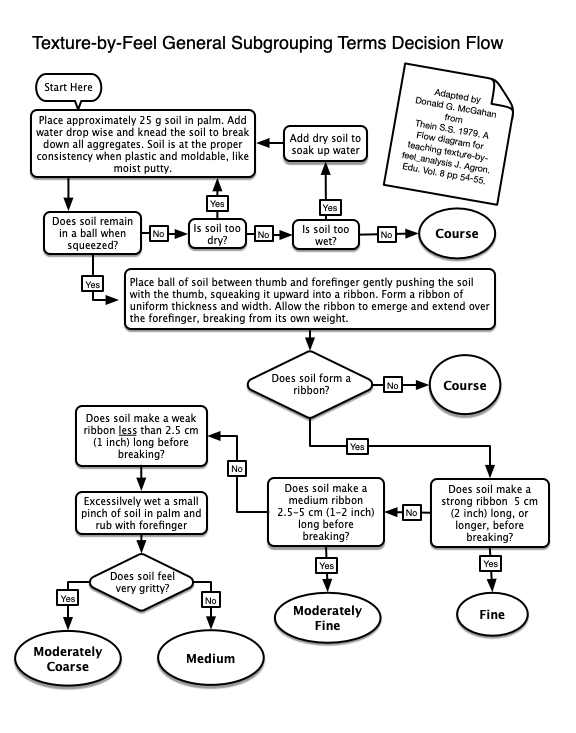
\includegraphics[width=0.98\columnwidth]{images/Texture_by_feel_analysis_DecissionTree-5-Category-bw-72pxpin-576x737px.png}
    \caption{Texture-by-Feel decision flow chart to determine one of the five General Textural Subgroups. Figure: Donald G. McGahan Creative Commons Attribution-ShareAlike-4.0-International.}
    \label{fig:TextureByFeelFlowChart5class}
\end{figure*}

% the above adapted figure is similar to an adaption of an 11 class by others e.g. USDA-NRCS \href{https://www.nrcs.usda.gov/wps/portal/nrcs/detail/soils/edu/?cid=nrcs142p2_054311}{https://www.nrcs.usda.gov/wps/portal/nrcs/detail/soils/edu/?cid=nrcs142p2_054311} NOT SURE ABOUT attaining permissions.

Post secondary High School FFA Land Judging teams determine a texture from the five general textural subgroup list for placing soils in a significantly simplified technical classification patterned after \textit{Land Capability Classification}. The three terms of the \textit{general texture group} are frequently further divided into the five \textit{general texture subgroup(s)}. These general textural subgroup terms are also not the same as the basic textural classes. A modified decision tree to choose one of the five general texture subgroup terms is presented in a texture-by-feel decision flow diagram (Figure \ref{fig:TextureByFeelFlowChart5class}).

High-school FFA Land Judgers and Homesite Judgers learn and employ the five general texture \textit{subgroups} wherein \textbf{\textit{fine}} is the correct general textural subgrouping term. Fine includes the basic textural class categories of \textit{clay}, \textit{sandy clay}, and \textit{silty clay}. The term \textit{fine} and the general textural group term \textit{clayey} actually includes the same basic textural class categories \textit{clay}, \textit{sandy clay}, and \textit{silty clay}. Similarly, the \textit{sand} and \textit{loamy sand} classes from the twelve basic category system become \textbf{\textit{coarse}} from the general texture subgrouping, or \textit{sandy} from the general texture grouping. Figure \ref{fig:TextureClass12-5-3} depicts the relationships between the the twelve basic textural classes and the general textural group and subgroup graphically.
    
\begin{figure*}
    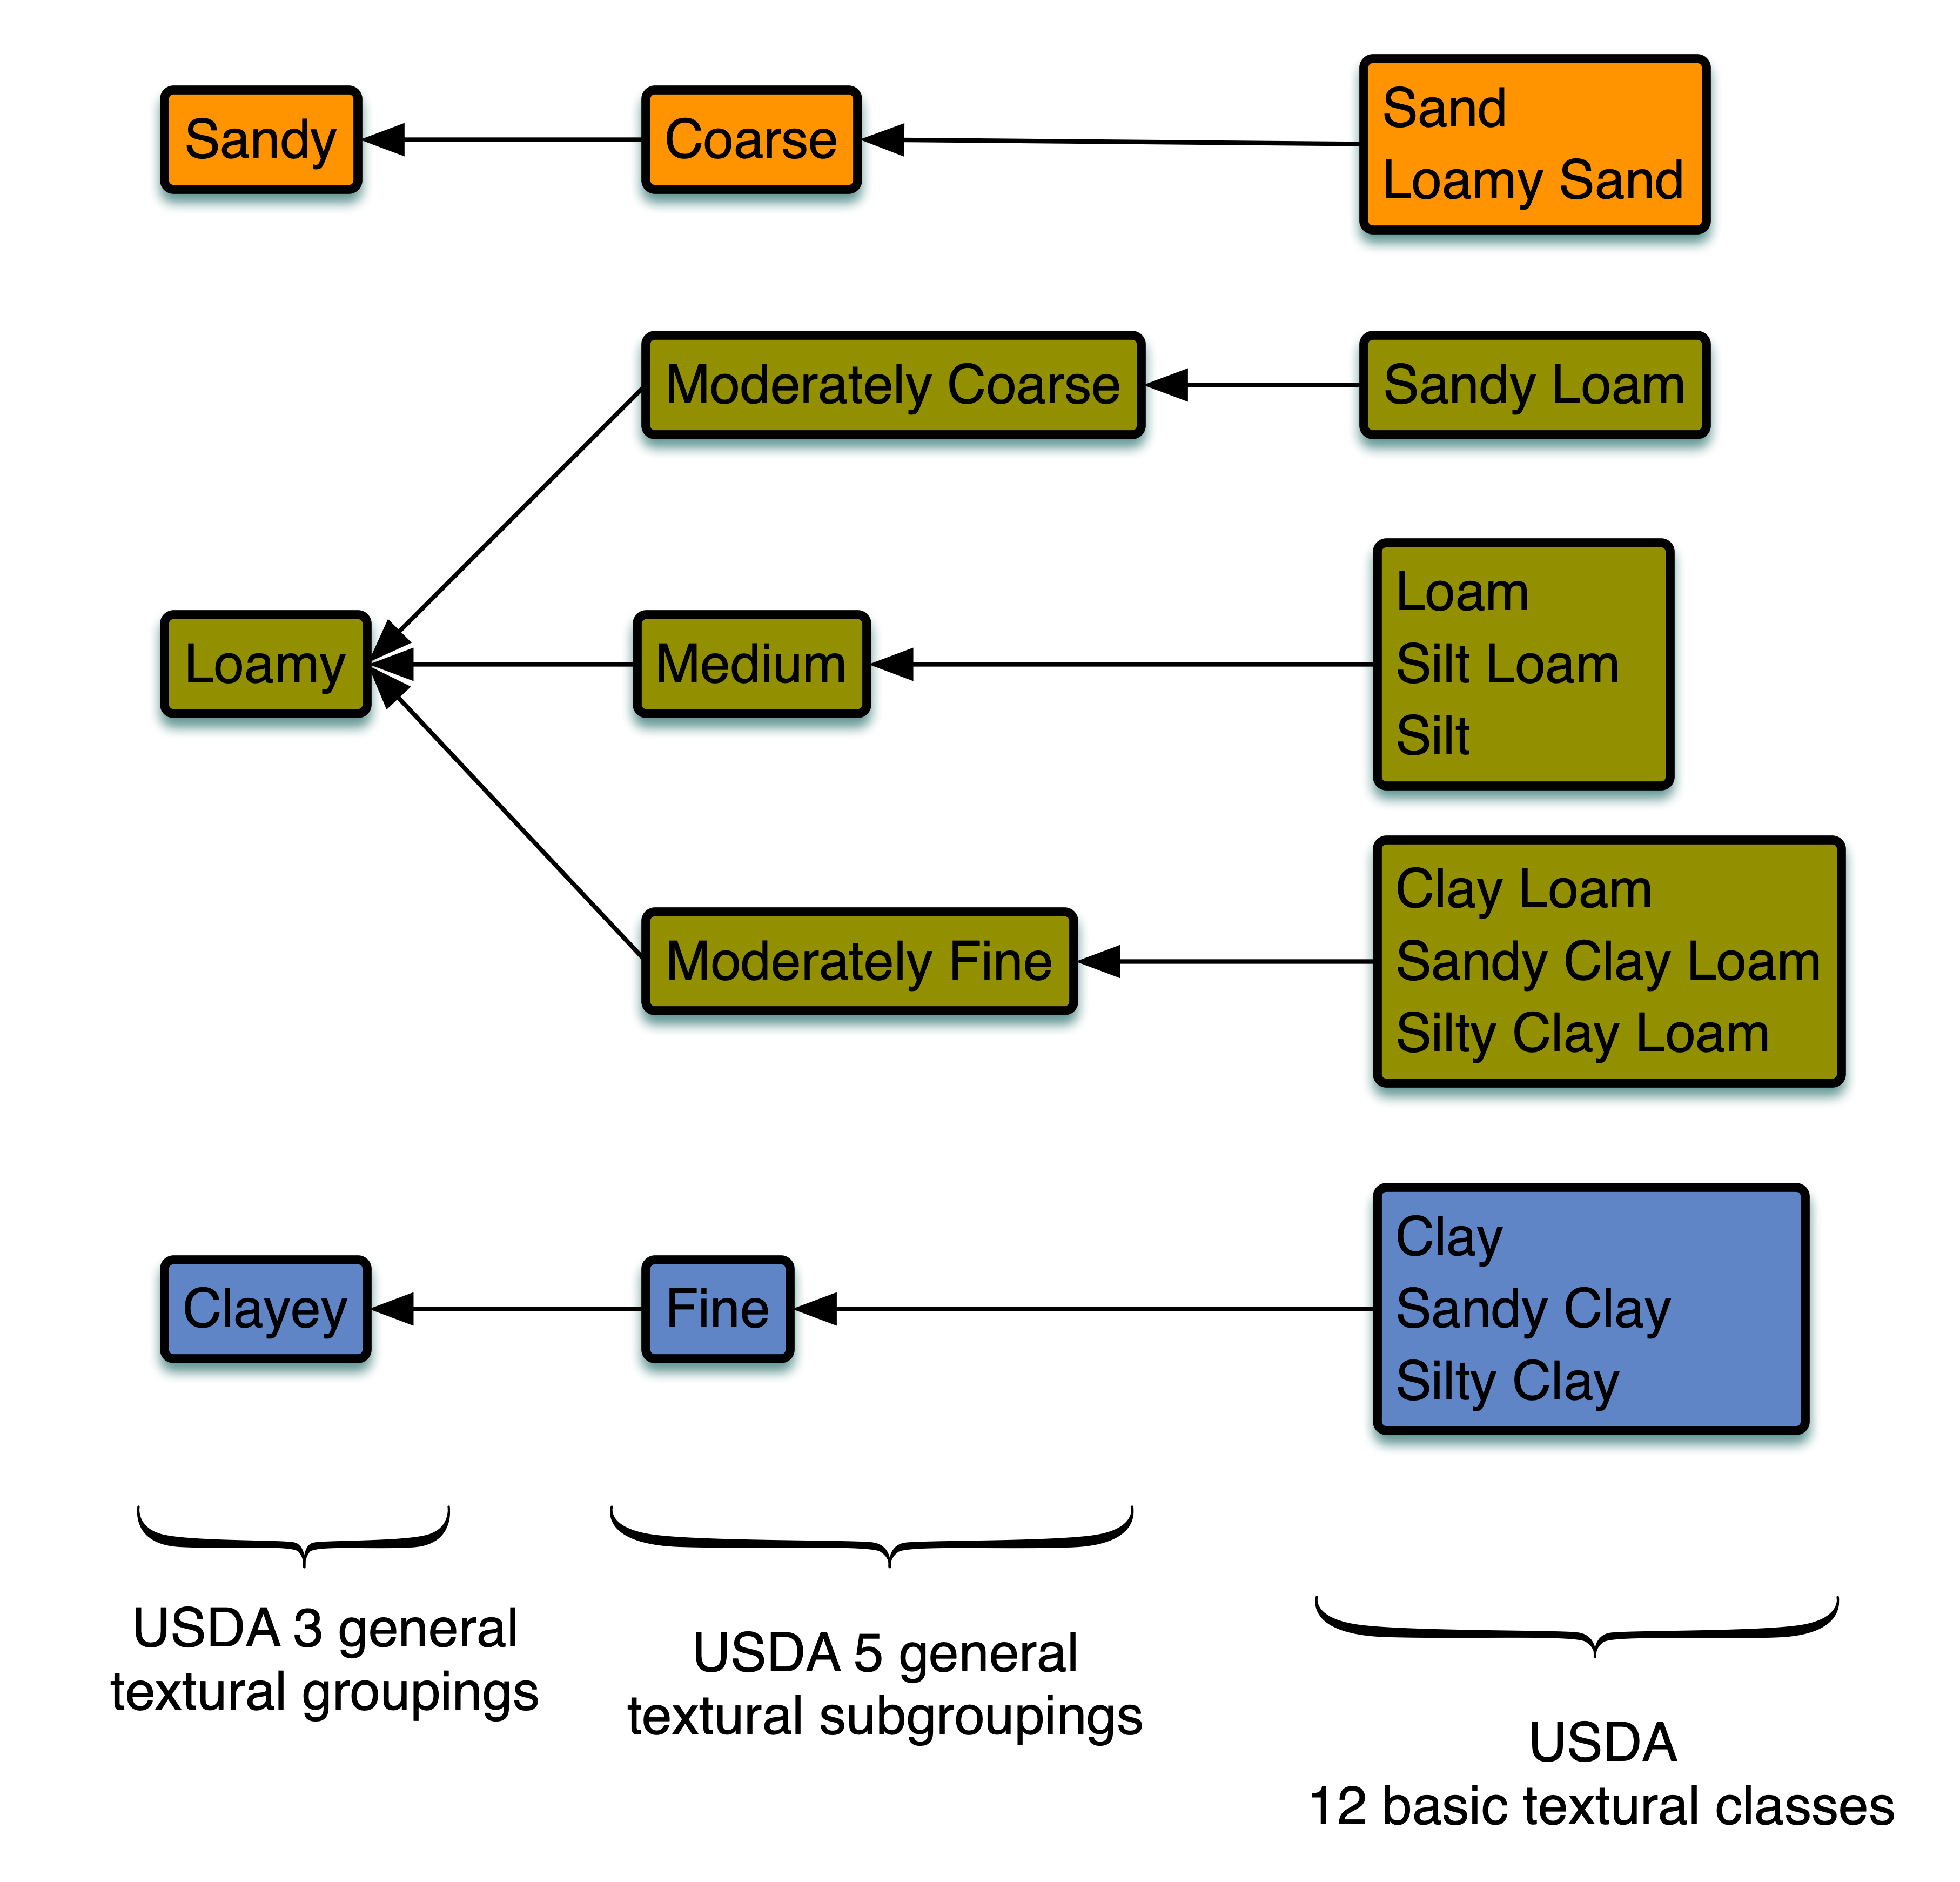
\includegraphics[width=0.98\columnwidth]
       {images/Textural_Classes_et_groupings_labeled-600dpi.png}
    \caption{Diagram relating the twelve basic textural classes, the five general texture subgroups and the three general texture groups. The High School organization FFA uses the USDA five general texture subgroups for their Career Development Events. Figure: Donald G. McGahan Creative Commons Attribution-ShareAlike-4.0-International.}
    \label{fig:TextureClass12-5-3}
\end{figure*}

\begin{figure}
    \centering
    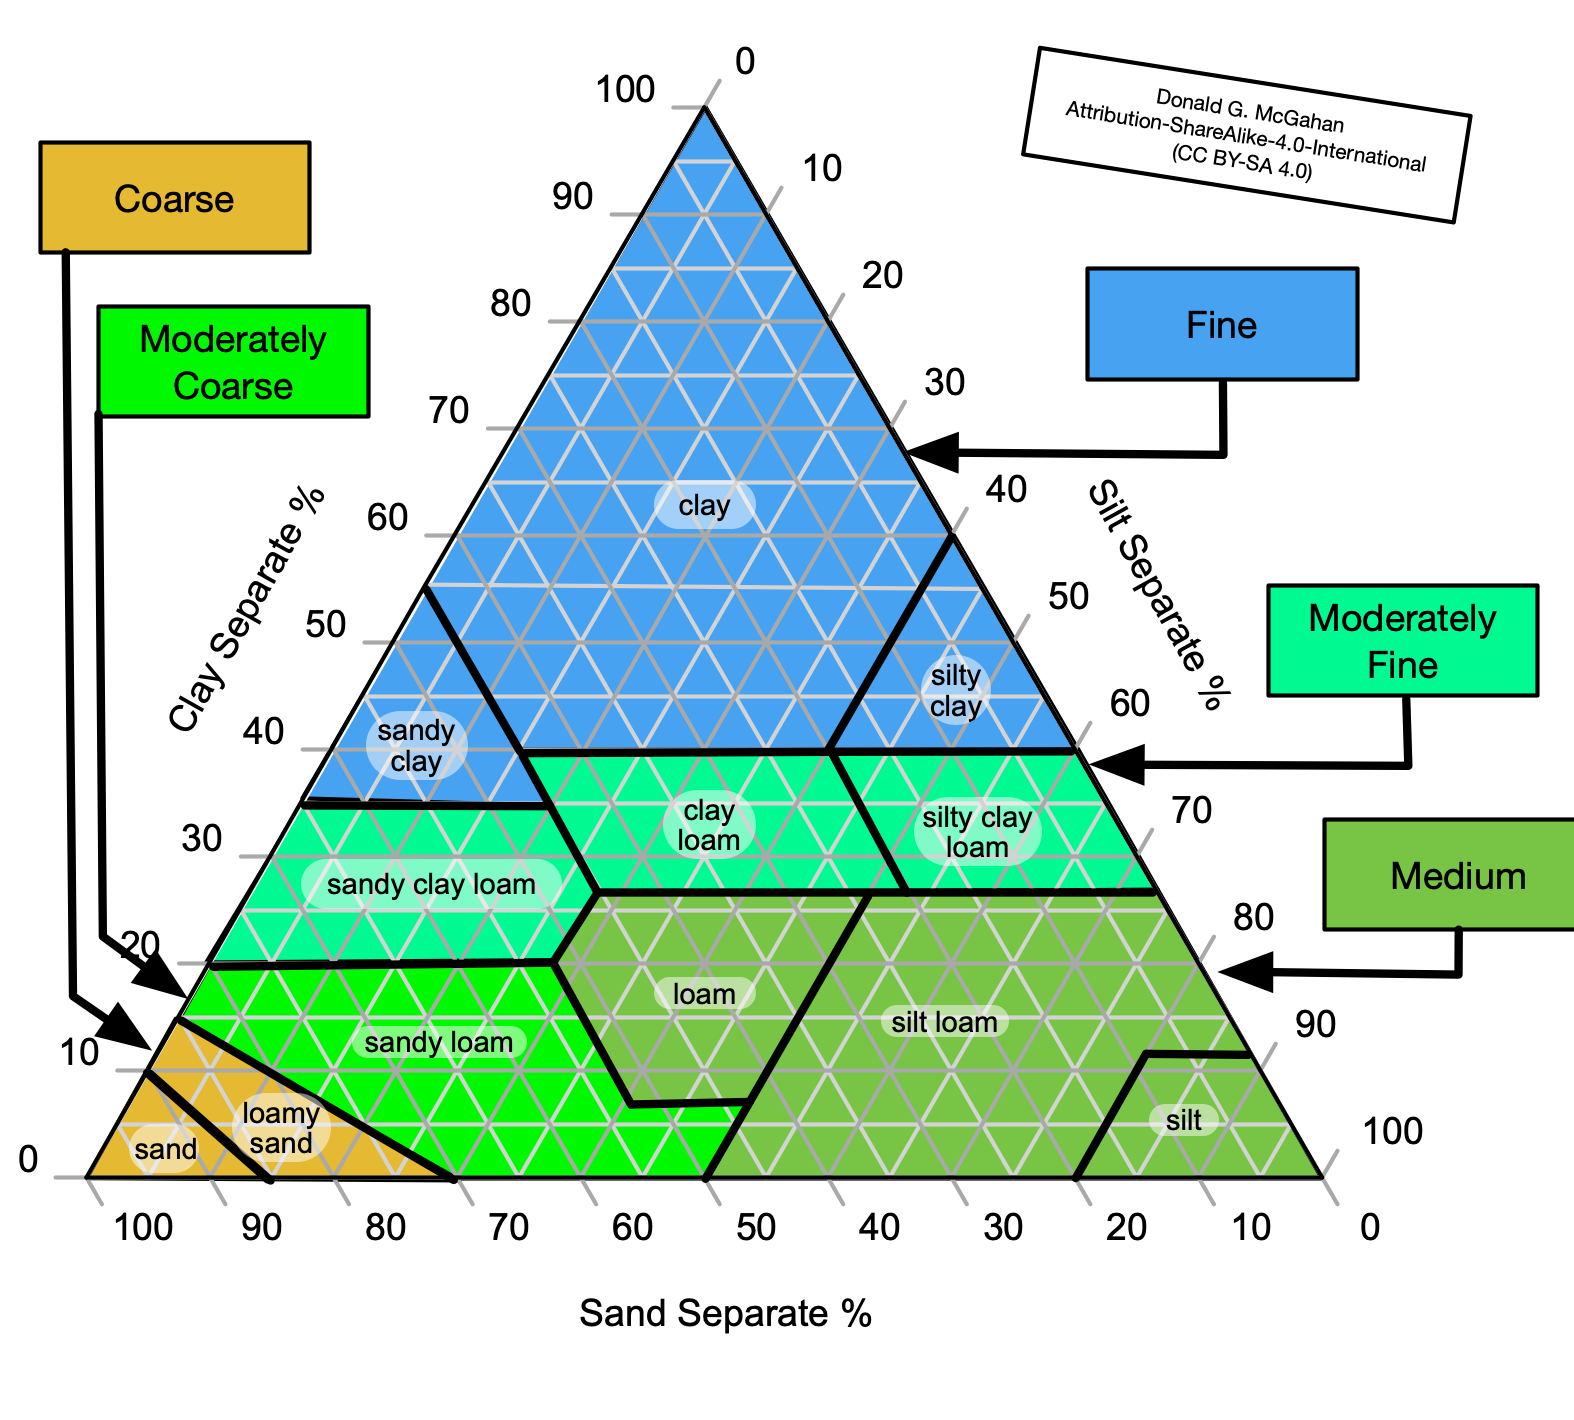
\includegraphics[width=0.98\columnwidth]{images/Textural_Triangle-w-subgrouping.png}
    \caption{The twelve basic textural class with color overlays corresponding to the five general textural subgroupings. These general textural subgroupings are used in FFA Land Evaluation and Homesite Career Development Events. Figure: Donald G. McGahan Creative Commons Attribution-ShareAlike-4.0-International.}
    \label{fig:textureTriangleWithsubgroupingOverlay}
\end{figure}

From a practical operative standpoint it seems most logical to first master the twelve basic textural classes. Still, as stated previously the general subgroupings are presented and utilized by secondary school learners with dubious instruction for the basic textural classes.

\section{Soil Structure}
\label{structure}
    
\textbf{Structure} is the term used to convey the arrangement of size separates pedologically arranged into larger stable units called \textbf{aggregates}, or \textbf{peds}, in the soil and expressed as regularly repeating pattern of permanent cleavage planes in the soil mass. The soil aggregates cleave planes form due to repeated compression and contraction of soil particles which may be related to shrink/swell of clay, freeze-thaw cycles, root penetration through soil, animals (earth worm activity), etc. The relative mechanical and water stability of peds are variable and related to the aggregate promoting substance–organics, iron oxides, carbonates, clays, and/or silica. Organics can be from decomposed vegetative material and/or root polysaccharides exuded from roots.

Soils can be structureless expressing a single grain or cohesive nature. Cohesive structureless soils can produce \enquote{artificial}–not pedogenetically derived–\textbf{clods} when broken up by mechanical means. Clods are different–not synnomous–than using the term \textbf{fragment} as fragment is a term used to describe a piece of a broken pedogenetically formed structure, or ped.

\textbf{Nodules} and \textbf{concretions} are two other arrangements encountered that have formed in soils and while both are cemented spherical bodies without obvious crystals the concretions display layering inside when cleaved whereas nodules do not.

Structure influences water movement, heat transfer, aeration, voids distribution, and erosion as a secondary influence to the overarching constraints and influences arising due to the soil texture. Unlike soil texture, however, soil structure can be changed by management practices.

Soil structure is observed, measured, and recorded in-situ as \textbf{Type}, \textbf{Grade}, and \textbf{Size}.
    
\subsection{Type of Structure}
    
Classing soil structure is first expressed by the form now called type and formally referred to as shape. Eight types exist: granular, angular blocky, sub-angular blocky, lenticular, platy, wedge, prismatic, and columnar (Figure \ref{fig:SoilStructureTypes}).

The prismatic and columnar type structure are taller than wide with the prismatic having flat tops and columnar having rounded tops that are commonly described as having \enquote{bleached} tops. The bleached tops result from dispersion and removal of pigmenting agents such as iron and manganese oxides and organic matters that so often adorn the outside of peds.

Granular and blocky structural types are roughly equidistant side to side and top to bottom. Granular are polyhedral with irregular faces that are difficult to imagine as clear nesting faces with their neighbors. Blocky structures planar faces are discernible as nesting with neighboring blocks. Angular describes blocky structure type with sharp angular faces versus the subangular blocky polyhedrals wherein the planar faces lack sharp angles and are subrounded.

Wedge type structure is elliptical and terminate at acute angles, often \ang{30}, or \ang{60}, with slickenside bounding edges. While the wedge structure type does not require the soil be a U.S. Soil Taxonomy Vertisol Order, the Vertisol Order, and Vertic taxonomic subgroups must include wedge type structure. For more on U.S. Soil Taxonomy seek a separate treatise. % dig-soilman: awaiting authoring a treatise on "Classification" for reference to that treatise.

Lenticular type structure is overlapping, lens-shaped peds that are generally parallel to the soil surface that are thick at the center and taper toward the edges and are formed by active or relic periglacial frost processes. They are most commonly described in soils with moderate to high water-holding capacity in moist conditions.

Platy type structure are flat plate like units that are wider than tall.

\begin{figure}
    \centering
    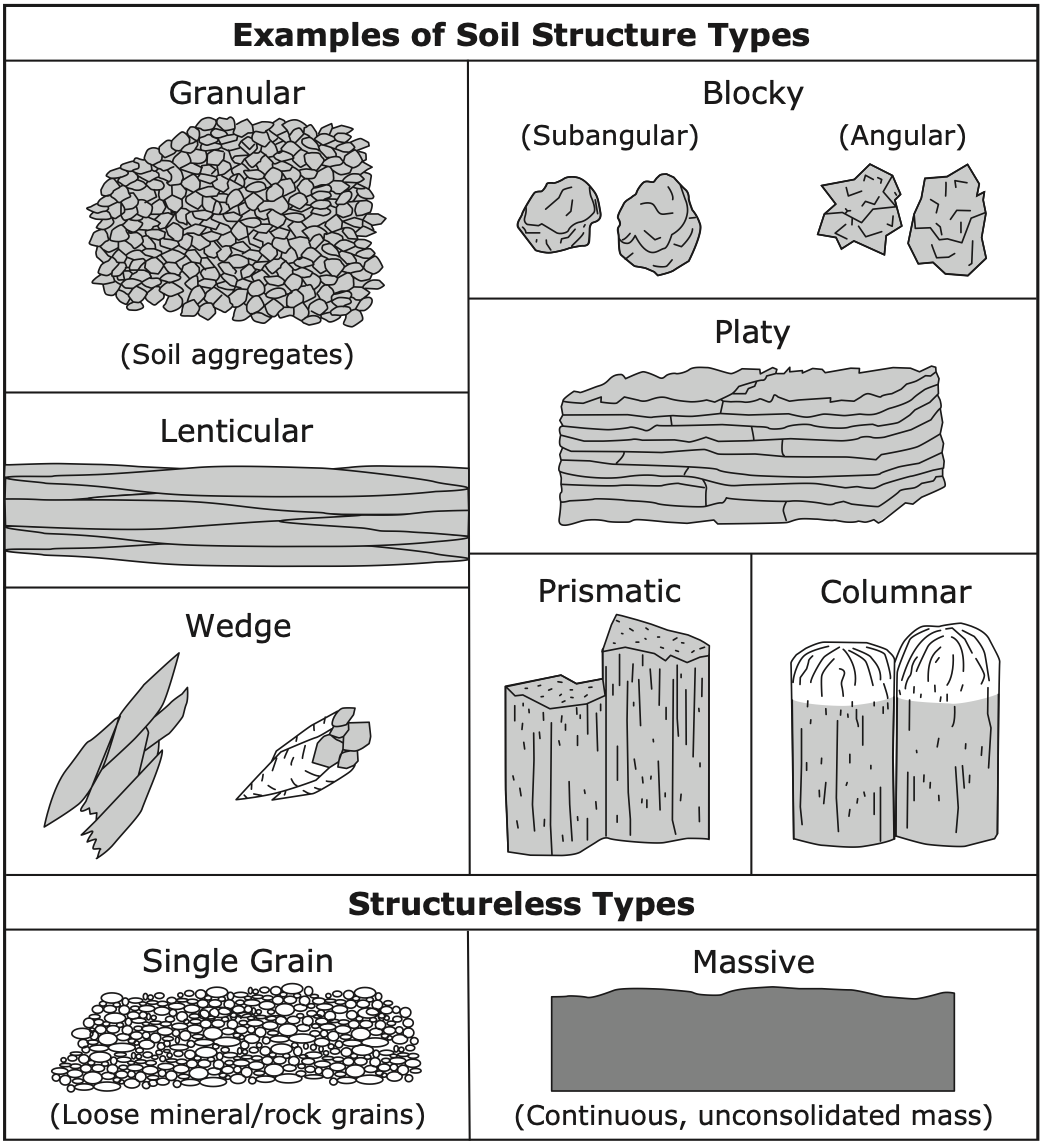
\includegraphics[width=0.98\columnwidth]{images/FieldBookVer3_ExamplesSoilStructureTypes1045x1145.png}
    \caption{Types of Soil Structure. From Soil Survey Staff 2012 Field Book for Describing and Sampling Soils version 3.}
    \label{fig:SoilStructureTypes}
\end{figure}

\subsection{Grade of Structure}
    
Three grades of structure are described.

\begin{itemize}
    \item \textbf{\textit{Weak}}: Peds are barely distinguishable in part of the \textit{moist} soil; only a few distinct peds can be separated from the soil mass.
    \item \textbf{\textit{Moderate}}: Peds are visible in place; many can be handled without breaking.
    \item \textbf{\textit{Strong}}: Most of the soil mass is visible as peds, moist of which can be handled with ease without breaking.
\end{itemize}

Soil structure may exist as a compound structure in which large peds may further fall apart into smaller blocks or smaller peds. Both are described starting with the larger type the term \enquote{parting to} and then the smaller type added to the description.
    
\subsection{Size of Structure}
    
Size is conveyed in such a way that the peds narrowest dimension  determines the size class for each type. Size classes for granular, angular blocky, sub-angular blocky, lenticular, wedge, prismatic, and columnar structure types are \textit{very fine}, \textit{fine}, \textit{medium}, \textit{coarse}, and \textit{very coarse}. For the platy structure type \textit{thin} is substituted for \textit{fine} and \textit{thick} is substituted for \textit{coarse} size class names.

The five size classes for granular and platy structures are \qty{< 1}{\milli\meter}, \qtyrange{1}{< 2}{\milli\meter}, \qtyrange{2}{< 5}{\milli\meter}, \qtyrange{5}{< 10}{\milli\meter}, and \qty{\geq 10}{\milli\meter}.

The six size classes for columnar, prismatic, wedge are \qty{< 10}{mm}, \qtyrange{10}{< 20}{mm}, \qtyrange{20}{< 50}{mm}, \qtyrange{50}{< 100}{mm}, \qtyrange{100}{< 500}{mm}, and \qty{\ge 500}{mm}. Note that these structures have this additional larger size class of extremely coarse that is not used with granular, platy, blocky, or lenticular structural types.

The five size class for angular and subangluar blocky and lenticular structure are \qty{< 5}{mm}, \qtyrange{5}{< 10}{mm}, \qtyrange{10}{< 20}{mm}, \qtyrange{20}{< 50}{mm}, and \qty{\ge 50}{mm}.

\begin{table}[!htbp]
\label{tab:astructuresizeclass}
\centering
\caption{Structure size classes.}
\begin{tabular}{ m{12em} m{5.5em} m{5.5em} m{5.5em} } \\[0.75em]
Size Class & \multicolumn{3}{c}{Criteria: Structural unit size (mm)} \\[0.75em] 
\cline{2-4} \\
& Granular \mbox{(Diameter)}, Platy \mbox{(Thickness)} & Columnar, Prismatic, Wedge, \mbox{(Diameter)} & Angular \& Subangular Blocky and Lenticular, \mbox{(Diameter)} \\[0.75em]
 \hline\\
{Very Fine, \mbox{(Very Thin)}} & \hfil \textless 1 &  \hfil\textless 10 &  \hfil\textless 5 \\[0.75em]
Fine, \mbox{(Thin)} & \hfil 1 to \textless 2 & \hfil 10 to \textless 20 & \hfil 5 to \textless 10 \\[0.75em]
{Medium, \mbox{(Medium)}} & \hfil 2 to \textless 5 & \hfil 20 to \textless 50 & \hfil 10 to \textless 20 \\[0.75em]
{Coarse, \mbox{(Thick)}} & \hfil 5 to \textless 10 & \hfil 50 to \textless 100 & \hfil \textless 20 to \textless 50 \\[0.75em]
{Very Coarse, \mbox{(Very Thick)}} & \hfil $\geq$ 10 & \hfil 100 to \textless 500 & \hfil $\geq$ 50 \\[0.75em]
{Extremely Coarse} & \hfil \textendash & \hfil $\geq$ 500 & \hfil \textendash \\[0.75em]
\hline
\end{tabular}
\end{table}

% dig-soilman: below is an html rendering of the above table.
%<table id="tab:astructuresizeclass">
%	<caption>Table Structure size classes.</caption>
%<tbody>
%	<tr class="odd">
%		<th rowspan="2" style="text-align: left;">Size Class</th>
%		<th colspan="3" style="text-align: center;">Criteria: Structural unit size (mm)</th>
%	</tr>
%	<tr class="even">
%		<th style="text-align: center;">Granular, (Diameter) Platy (Thickness)</th>
%		<th style="text-align: center;">Columnar, Prismatic, Wedge, (Diameter)</th>
%		<th style="text-align: center;">Angular &amp; Subangular Blocky and Lenticular, (Diameter)</th>
%	</tr>
%	<tr class="odd">
%		<td style="text-align: left;">Very Fine (Very Thin)</td>
%		<td style="text-align: center;">&lt; 1</td>
%		<td style="text-align: center;">&lt; 10</td>
%		<td style="text-align: center;">&lt; 5</td>
%	</tr>
%		<td style="text-align: center;">1 to &lt; 2</td>
%		<td style="text-align: center;">10 to  &lt;  20</td>
%		<td style="text-align: center;">5 to &lt; 10</td>
%	</tr>
%	<tr class="odd">
%		<td style="text-align: left;">Medium (Medium)</td>
%		<td style="text-align: center;">2 to &lt; 5</td>
%		<td style="text-align: center;">20 to &lt; 50</td>
%		<td style="text-align: center;">10 to &lt; 20</td>
%	</tr>
%		<tr class="even">
%		<td style="text-align: left;">Coarse (Thick)</td>
%		<td style="text-align: center;">5 to &lt;  10</td>
%		<td style="text-align: center;">50 to &lt; 100</td>
%		<td style="text-align: center;">20 to &lt; 50</td>
%	</tr>
%	<tr class="odd">
%		<td style="text-align: left;">Very Coarse (Very Thick)</td>
%		<td style="text-align: center;">&ge; 10</td>
%		<td style="text-align: center;">100 to &lt; 500</td>
%		<td style="text-align: center;">&ge; 50</td>
%	</tr>
%		<tr class="even">
%		<td style="text-align: left;">Extreamly Coarse</td>
%		<td style="text-align: center;">&ndash;</td>
%		<td style="text-align: center;">&ge; 500</td>
%		<td style="text-align: center;">&ndash;</td>
%	</tr>
%</tbody>
%</table>

\subsection{Destruction of Aggregates}
    
Increasing sodium tends to speed structure degradation. The sodium interacts with the soil particles promoting dispersion. Dispersed size separates are frequently in clay size class and greatly diminish the movement of water and this limits the removal of salts. Tillage also destroys structure and though it can temporarily fluff up the size separates it tends to promote the decomposition of organic matter and the organic matter, as stated previously, is an aggregating agent that promotes structure stability. Trafficking by animals and machinery also have a negative impact on soil structure.
    
\section{Density}
\label{density}
    
Solids Density $\left(\rho_s\right)$ is the density of the solid soil particles only in units of mass per volume e.g., (\unit{\gram\per\cubic\centi\metre}). Often in texts the Greek letter rho $\left(\rho\right)$ is a shorthand symbol for density and s is for solids.

\begin{equation}
    Particle\,Density = \left(\frac{Weight\,of\,Solids}{Volume\,of\,Solids}\right)   
\end{equation}

Expressed in a maths form $\rho_p =\frac{W_s}{V_s}$ where $\rho$ is density, $p$ is particle, $W$ is weight, $V$ is volume, and $s$ is solid.

Range of particle density values for typical soil materials varies with inorganic materials ranging from \numrange{2.6}{2.75} \unit{\gram\per\cubic\centi\metre}.

For inorganic materials $\rho_s$ is  (Al =
	\qty[per-mode=symbol]{27}{\gram\per\mole}; Si = 
	\qty[per-mode=symbol]{28}{\gram\per\mole}; and Fe =
	\qty[per-mode=symbol]{56}{\gram\per\mole}). For organic materials
	$\rho_s$ is  (C = \qty[per-mode=symbol]{12}{\gram\per\mole}; O =
	\qty[per-mode=symbol]{16}{\gram\per\mole}; and H =
	\qty[per-mode=symbol]{1}{\gram\per\mole}).

The $\rho_s$ is affected by the kind of minerals or rock (e.g., iron is heavier than aluminum) and the proportion of organic matter to mineral (inorganic) material.

The $\rho_s$ is not affected by texture or soil structure (arrangement of soil solids).

Bulk Density $\left(\rho_b\right)$ is a measure of the weight of the soil per unit volume. Volume includes both solids and pore space. Usually reported as the weight of oven-dry soil following heating to \qty{110}{\degreeCelsius}.

\begin{equation}
    Bulk\,Density =    	\left(\frac{Weight\,of\,Oven\,Dry\,Soil}{Volume\,of\,Soil\,Sampled}\right)
\end{equation}

\noindent\begin{minipage}{\textwidth}
For maths treatment:

\begin{equation}
    \rho_b = \frac{M_s}{V_t}\quad
\end{equation}
\begin{equation*}
    \begin{aligned}
    \text{where:}.                    \\
        \rho_b &= \text{density bulk} \\
        M_s &= \text{mass of solids}  \\
        V_t &= \text{volume total}
    \end{aligned}
\end{equation*}
\end{minipage}

The $\rho_b$ values for most mineral (inorganic) soils are \qtyrange[range-units=single]{1.20}{1.40}{\gram\per\cubic\cm} and for organic soils \qtyrange[range-units=single]{0.10}{0.25}{\gram\per\cubic\centi\meter}. Recall that the specific gravity (density) of water, at STP, is \qty[per-mode=fraction]{1.00}{\gram\per\cubic\centi\meter}.

Bulk Density is affected by:
\begin{itemize}
    \item Particle density; $\left(\rho_s\right)$  
    \item Texture because it affects total volume of the voids
	$\left(V_v\right)$, or porosity $\left(\eta\right)$: 
	$\text{sand}\,\rho_{\text{b}} < \text{clay}\,\rho_{\text{b}}$ \item Soil
	structure because it also affects porosity $\left(\eta\right)$;
	$\uparrow$  structure generally $\uparrow\,\eta$ \item Concentration of
	organic matter – affects $\rho_s$ and porosity $\left(\eta\right)$ \item
	Cultivation – tends to result in both compaction and destruction of
	organic matter.  
\end{itemize}

% ToDo dig-soilman: Cultivation and compaction can be addressed here a bit, and then also in a chapter of engineering and erosion or no? For now no.

\section{Voids}
\label{voids}

The voids that arise owing to the size and irregular shape of the soils size separates exist in what can be termed the \textbf{matrix}. Some writings will refer to these as intraaggregate voids though this assumes that aggregation currently exists. An a-pedal\textemdash{}structureless\textemdash{}soil matrix also includes these voids in the matrix. The aggregation of the size separates that favor the repeating planes of separation between the peds\textemdash{}orientated aggregates\textemdash{}are known to often result in larger diameter voids. The formation of structural units and the resulting repeating planes of separation tend to increase the relative proportion of void to solid and the term interaggregate voids is often applied to the voids between the 'structural' ped units. These voids between peds together with voids created by burrowing arthropods, abandoned root channels, and voids caused by entrapped gasses as a result of water movement can be considered \textbf{nonmatrix voids}. Nonmatrix voids are not only generally larger in cross section than matrix voids, but also can be considered more dynamic in their fluid occupancy: air and/or water.  

% dig-soilman: when Soil Climate–water combined with temperature–treatise is written the fluid occupancy portion should expand on the passage below and a reference can be properly placed in the below text.
% dig-soilman> When Soil Biology treatise is written the below paragraph can be edited to cite it directly.

This fluid occupancy is of particular interest since both air and water contents are of great interest to biologicals. The occupancy of the voids by water is a storage medium that is critical to biologicals. The movement of the water and the solutes in the water is also of import to the biologicals. For more on the storage and movement of water and interaction with biologicals seek other treatises.

The proportion of air in the voids is critical to aerobic biologicals\textemdash{}plants, arthropods, and numerous microorganisms\textemdash{}and the soil air relative composition is, in turn, partially controlled by void diameter.

Classification categories of voids are based on their effective diameter, or size. The basis of the following presented classification is soil water\textemdash{}plant relationships.

\textbf{\textit{Macrovoids}} are \qty{> 75}{\micro\metre} and was chosen utilizing empirical data wherein tensions of $\leq$ \qty{40}{\centi\meter} ($\leq$ \qty{-4}{kPa}) led to greater percolation rates. The emptying of macrovoids also leads to air exchange within the soil.

\textbf{\textit{Mesovoids}} are \qtyrange{30}{75}{\micro\metre} and when connected are important in transport and distribution of water. Mesovoids together with macrovoids are contributors to renewal and exchange of air in the soil.

\textbf{\textit{Microvoids}} \qtyrange{5}{30}{\micro\metre} and \textbf{\textit{ultramicrovoids}} \qtyrange{0.1}{5}{\micro\metre} are are voids most responsible for storage of water that is available to plants, as the habitat for microorganisims, and soil fauna.

\textbf{\textit{Cryptovoids}} \textless{} \qty{0.1}{\micro\metre} represent storage of water that is  unavailable to most plants. They are generally too small for roots and most microorganisms.

Void connectivity and tortuous paths between void tubules dictates the relative movement and connectivity of the air and water within the soil. Irregular effective diameters are quite common in soils and impede the filling and emptying of the voids.

The distribution of voids among the aforementioned void classifications as part of the total volume of voids has a meaningful impact on the soil system and the ecological process for which the soil system is so important. Except for the cryptopores the relative proportions of these classes can be impacted by management and soil health practices.

Of the four voids properties continuity, tortousity, size distribution, and total void volume the total void volume is perhaps most easily measured. A common measurement reported is porosity.

\section{Porosity}
\label{porosity}

Porosity $\left(\eta\right)$ is the fraction of soil volume occupied by air and water (non-solids). Soil porosities range from 0.30 to 0.60 (or \qty{30}{\percent} to \qty{60}{\percent}) for most soils. Note the difference between porosity $\left(\eta\right)$ or $\left(\phi\right)$ and percent porosity $\left(\%\,\eta\right)$ or $\left(\%\,\phi\right)$. \textit{Note}: While the lower case Greek letters eta $\left(\eta\right)$ and phi $\left(\phi\right)$ are most often applied as the variable for porosity any symbol can be applied. It is a reminder to define each variable when presenting relationships with variables. 

\noindent\begin{minipage}{\textwidth} 

A maths treatment of porosity is:

\begin{equation}
    \eta = \frac{\left(V_a + V_w\right)}{\left(V_a + V_w + V_s\right)}
\end{equation}

\begin{equation*}
    \begin{aligned}
        \text{where:}                              \\
        \eta &= \text{porosity (greek letter eta)} \\
        V_a &= \text{volume of air}                \\
        V_w &= \text{volume of water}              \\
        V_s &= \text{volume of solids}
    \end{aligned}
\end{equation*}
\end{minipage}

\noindent\begin{minipage}{\textwidth}
This can be simplified to:

\begin{equation}
    \eta = \frac{V_v}{V_t}
\end{equation}
\begin{equation*}
    \begin{aligned}
        \text{where:}                               \\
        \eta &= \text{porosity}                     \\
        V_v &= \text{volume of the voids}:\,V_a+V_w \\
        V_t &= \text{volume total}:\,V_a+V_w+Vs
    \end{aligned}
\end{equation*}
\end{minipage}

It can be challenging to determine the $V_v$ when the relative proportions of $V_a$ and $V_w$ are unknown. When $V_a = 0$ the soil is saturated. Saturating a known total volume $\left(V_t\right)$  such as a core extracted from a soil and massing the saturated soil is useful because the density of water, its specific gravity, is know to be \qty[per-mode = symbol]{1}{\gram\per\cubic\centi\metre}. Since $V_a=0$ then $V_w=V_v$. The same sample can then have the water driven off by heating in a \qty{110}{\degreeCelsius} oven until it no longer reduces in mass and the difference in mass equates to a volume of voids $\left(V_v\right)$ that the water occupied. This is useful because the particle density does not have to be measured.

 \begin{figure}
     \centering
     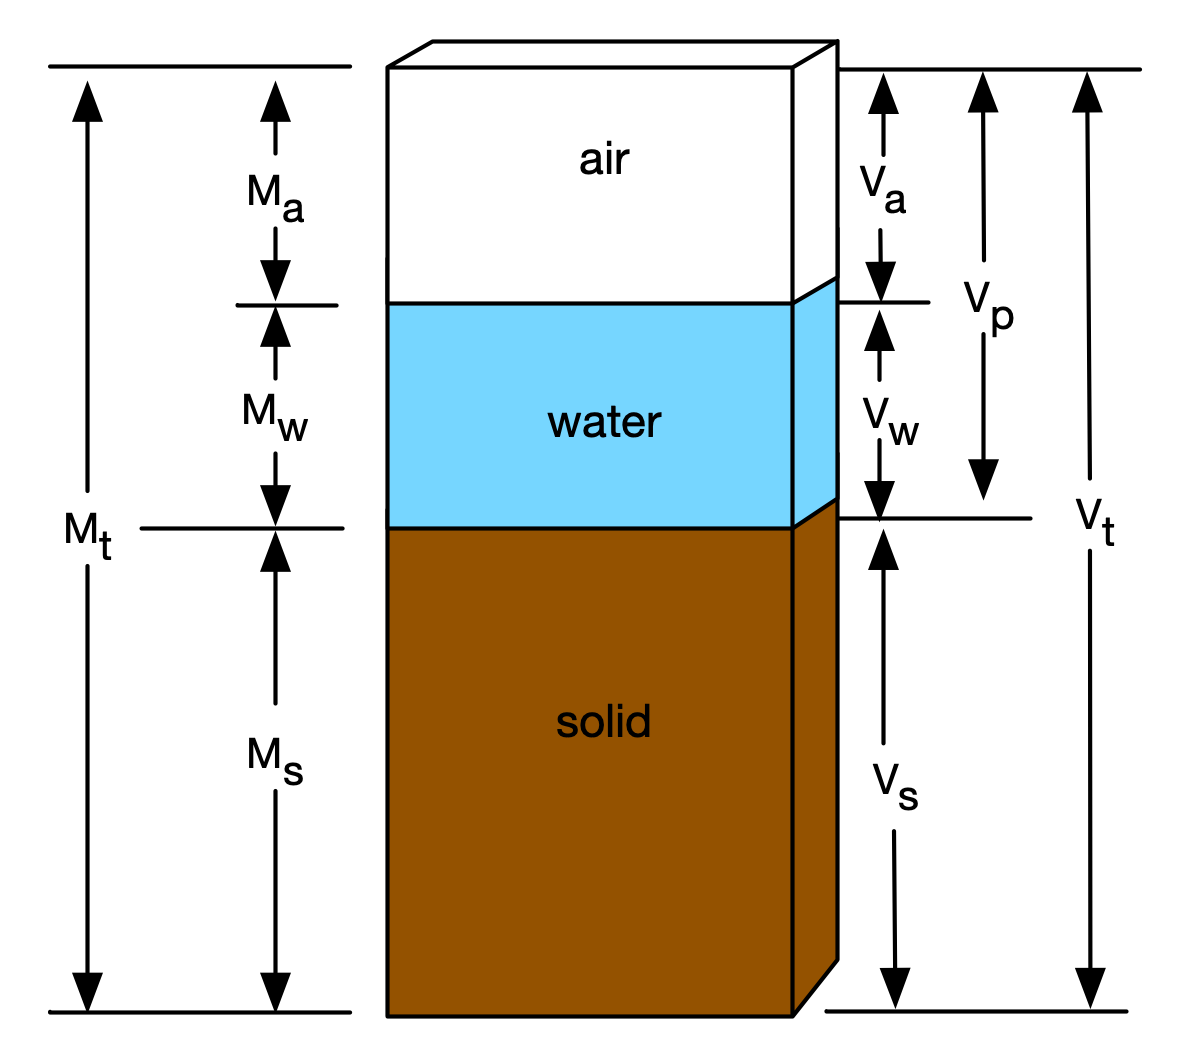
\includegraphics[width=0.75\columnwidth]{images/TallBox-ideal-soil-volume.png}
     \caption{Illustration of "idealized" soil volume occupied by voids and solids. The void volume is divided between air and water. The mass relationship is dominated by solids due to there greater density. Air contributes very little mass compared to water and solids. Figure: Donald G. McGahan Creative Commons Attribution-ShareAlike-4.0-International.}
     \label{fig:idealizedsoilvolumne}
 \end{figure}

Another estimate of porosity can be derived if the average solids density $\left(\rho_s\right)$ is known or estimated. Estimation of average solids density is frequently employed as a first estimate. Estimating average solids density is guided by empirical evidence and assumption that the dominate soil minerals might be quartz, feldspars, micas, and secondary clays. The solids density of \qty[per-mode = symbol]{2.65}{\gram\per\cubic\centi\metre} is most frequently adopted when the average solids density is not measured.

The quotient of bulk density $\left(\rho_b\right)$ to solids density $\left(\rho_s\right)$ for soil should always be a value less than one and represents the fraction of the whole soil that is occupied by the solids. When subtracted from the whole the quotient of bulk density to solids density will yield the fraction of the whole soil that is voids.

\noindent\begin{minipage}{\textwidth}
\begin{equation}
    \eta =\left(1-\frac{\rho_{\text{b}}}{\rho_{\text{s}}}\right)
\end{equation}
\begin{equation*}
    \begin{aligned}
        \text{where:}                                            \\
        \eta &= \text{porosity or void fraction of the whole }.  \\
        \rho_b &= \text{density of bulk soil}                    \\
        \rho_s &= \text{density of solids}                       \\
        1 &= \text{the whole}
    \end{aligned}
\end{equation*}
\end{minipage}

Porosity as a percent:

\noindent\begin{minipage}{\textwidth}
\begin{equation}
    \%\,\eta =\left(1-\frac{\rho_{\text{b}}}{\rho_{\text{s}}}\right) \times 100
\end{equation}
\begin{equation*}
    \begin{aligned}
        \text{where:}                                          \\
        \eta &= \text{porosity or void fraction of the whole } \\
        \rho_b &= \text{density of bulk soil}                  \\
        \rho_s &= \text{density of solids}                     \\
        1 &= \text{the whole}
    \end{aligned}
\end{equation*}
\end{minipage}

Example:

What is the percent porosity of a soil where $\rho_b = \qty[per-mode=fraction]{1.80}{\gram\per\cubic\centi\meter}$ and $\rho_s = \qty[per-mode=fraction]{2.65}{\gram\per\cubic\centi\meter} ?$ \\
$\%\,\eta = 32$

Porosity varies with texture, structure, and bulk density. Soils with more clay tend to have greater porosity than soils where sands dominate the size separates.

Porosity and bulk density are inversely related and can be related with maths as:

\noindent\begin{minipage}{\textwidth}
\begin{equation}
    \eta \, \frac{1}{\propto} \, \rho_b
\end{equation}

\begin{equation*}
    \begin{aligned}
        \text{where:}                                          \\
        \eta &= \text{porosity or void fraction of the whole } \\
        \rho_b &= \text{density of bulk soil}                  \\
        \propto &= \text{proportional to}                      \\
        \frac{1}{\propto} &= \text{inversely proportional to}
    \end{aligned}
\end{equation*}
\end{minipage}

Decreasing bulk density promotes porosity. The pores are the voids between the solids that can contain air and or water. Biologicals in the soil rely on water stored their and aerobic organisms rely of the air composition.

When discussing pores it is frequently useful to group pores by the classes of void diameter(s) where macro- is applied to voids with a diameter greater than \num{> 0.075}{mm} and meso- or micro- having a diameter \num{< 0.075}{mm}. As stated, the use of void diameters is useful because water and air move relatively rapidly through the voids connected together that are effectively macropores and much slower through smaller voids connected together that are effectively termed meso- or micropores. Still, the continuity of void diameter in soil are generally not linear and inter-connectivity between varying diameter voids impacts the movement of the fluids: air and water. Consider that when a grouping of connected macrovoids has a section of microvoids the microvoid section would constrain movement of water or air.

% dig-soilman: The following passage within the \textit{} refers another treatise that is not part of this treatise for addressing water in soils.

Porosity alone is insufficient to fully understand fluid movement in soils but coupling with textural class increases what can be inferred. Though the porosity is generally greater in a clay soil than a sand soil. But the average cross-section diameter of sandy soil matrix voids connected as pores are generally greater than the average cross-section diameter of clay soils. Thus, water and air flow more rapidly through sandy soils and more slowly through soils high in clay despite the greater overall porosity associated with the increase in content of clay in a soil. This is owing to the interaction of these fluids and the solids surfaces. \textit{For more on fluid interaction with solids seek a the treatise of soil climate and/or water in soils.}

In the preceding discussion voids and pores are defined separately. Pores can also be grouped into  general types in keeping with the types of voids. Interparticle pores are the connected void spaces occurring between the individual soil particles. Interaggregate pores are the connected void space occurring between soil aggregates. Biopores are pores created by biological activity (e.g., roots and earthworms).

Generally, in an overarching way, we can infer much regarding void diameter and textural class. It has been established above that the matrix pores of sandy soils are dominated more by macrovoids. Clay soils are more dominated by microvoids. Thus, in most instances water and air flow more rapidly through sandy soils and more slowly through soils higher in clay. This is despite soils with more clay having a higher overall proportion of voids: greater porosity. Reducing trafficking and mechanical disturbance of soils with greater clay content are practices that promote establishment and retention of interaggregate pores and therefore greater fluid movement.

\section{Soil Color}
\label{color}

% dig-soilman: figures are appropriate such as the page of a munsell colorbook and perhaps the relationship between hue, value, and chroma.

Most primary soil minerals are not highly colored (often light gray). A primary soil mineral are those that have not been altered chemically since they solidified from the molten magma. Soil color has great interpretive significance as it is indirectly related to many other soil properties, conditions, and processes.

% dig-soilman: The following passage refers to another treatise addressing soil chemistry and a reference should be inserted if they are bound.
Soil color is mostly due to the presence of materials that coat the surfaces of soil minerals. These materials coating the soil minerals could be organic materials or secondary soil minerals.

Soil organic materials consists of plant, animal and microbial residues in various stages of decomposition. The compounds that are more resistant to decay or those relatively protected from decay owing to their adsorption onto mineral soil surfaces are  collectively termed humus. A fraction of the humus consist of relatively higher weight but more amorphous compounds. It is these compounds that are influential in imparting a brown to black color to soils.

Recrystallized or modified products from the chemical breakdown and/or alteration of primary minerals are the origin of secondary soil minerals. Iron in primary minerals begin in their Fe-II reduced form. With exposure to water and air in the soil the iron is oxidized to Fe-III which in sufficient quantities results in rubification. See a treatise on soil chemistry for more. % Altering this last sentence to a treatise on "Soil Chemistry" and should have reference if the two are bound.

Alteration of reducing and oxidizing (redox) conditions seen when the soil is in well aerated conditions may be seen in the soil as zones of concentrations offset by zones of depletion. The inference of such might be that oxidized and depleted iron patterns, or redoximorphic condition, are a result of a cycling between being saturated with water, poor drainage, followed by more aerobic conditions, good drainage, these are some of the evidences of hydric soil conditions in that zone of the soil, and soil color are strong inferences toward such a hydric conditions.

Soil color determination is accomplished by matching soil to color chips in The Munsell Book of Color. Color is communicated in a letter and number combination. These describe three parts of color: hue, value, and chroma such as 10YR 5/4. \textbf{\textit{Hue}} is the dominant spectral wavelength such as the colors of the rainbow (ROYGBIV). Soil is frequently in the red-orange-yellow range. A 10R represents \qty{100}{\percent} whereas a 5Y represents \qty{75}{\percent} yellow and \qty{25}{\percent} red. \textbf{\textit{Value}} is the lightness of color. A value of 0 would be lowest lightness and 10 would be the lightest. \textbf{\textit{Chroma}} is the relative purity, intensity or strength of the hue. A chroma of 0 is pure black, grey, or white (hue dependent) (Figure \ref{fig:MunsellColorSystem}).

\begin{figure}
    \centering
   % 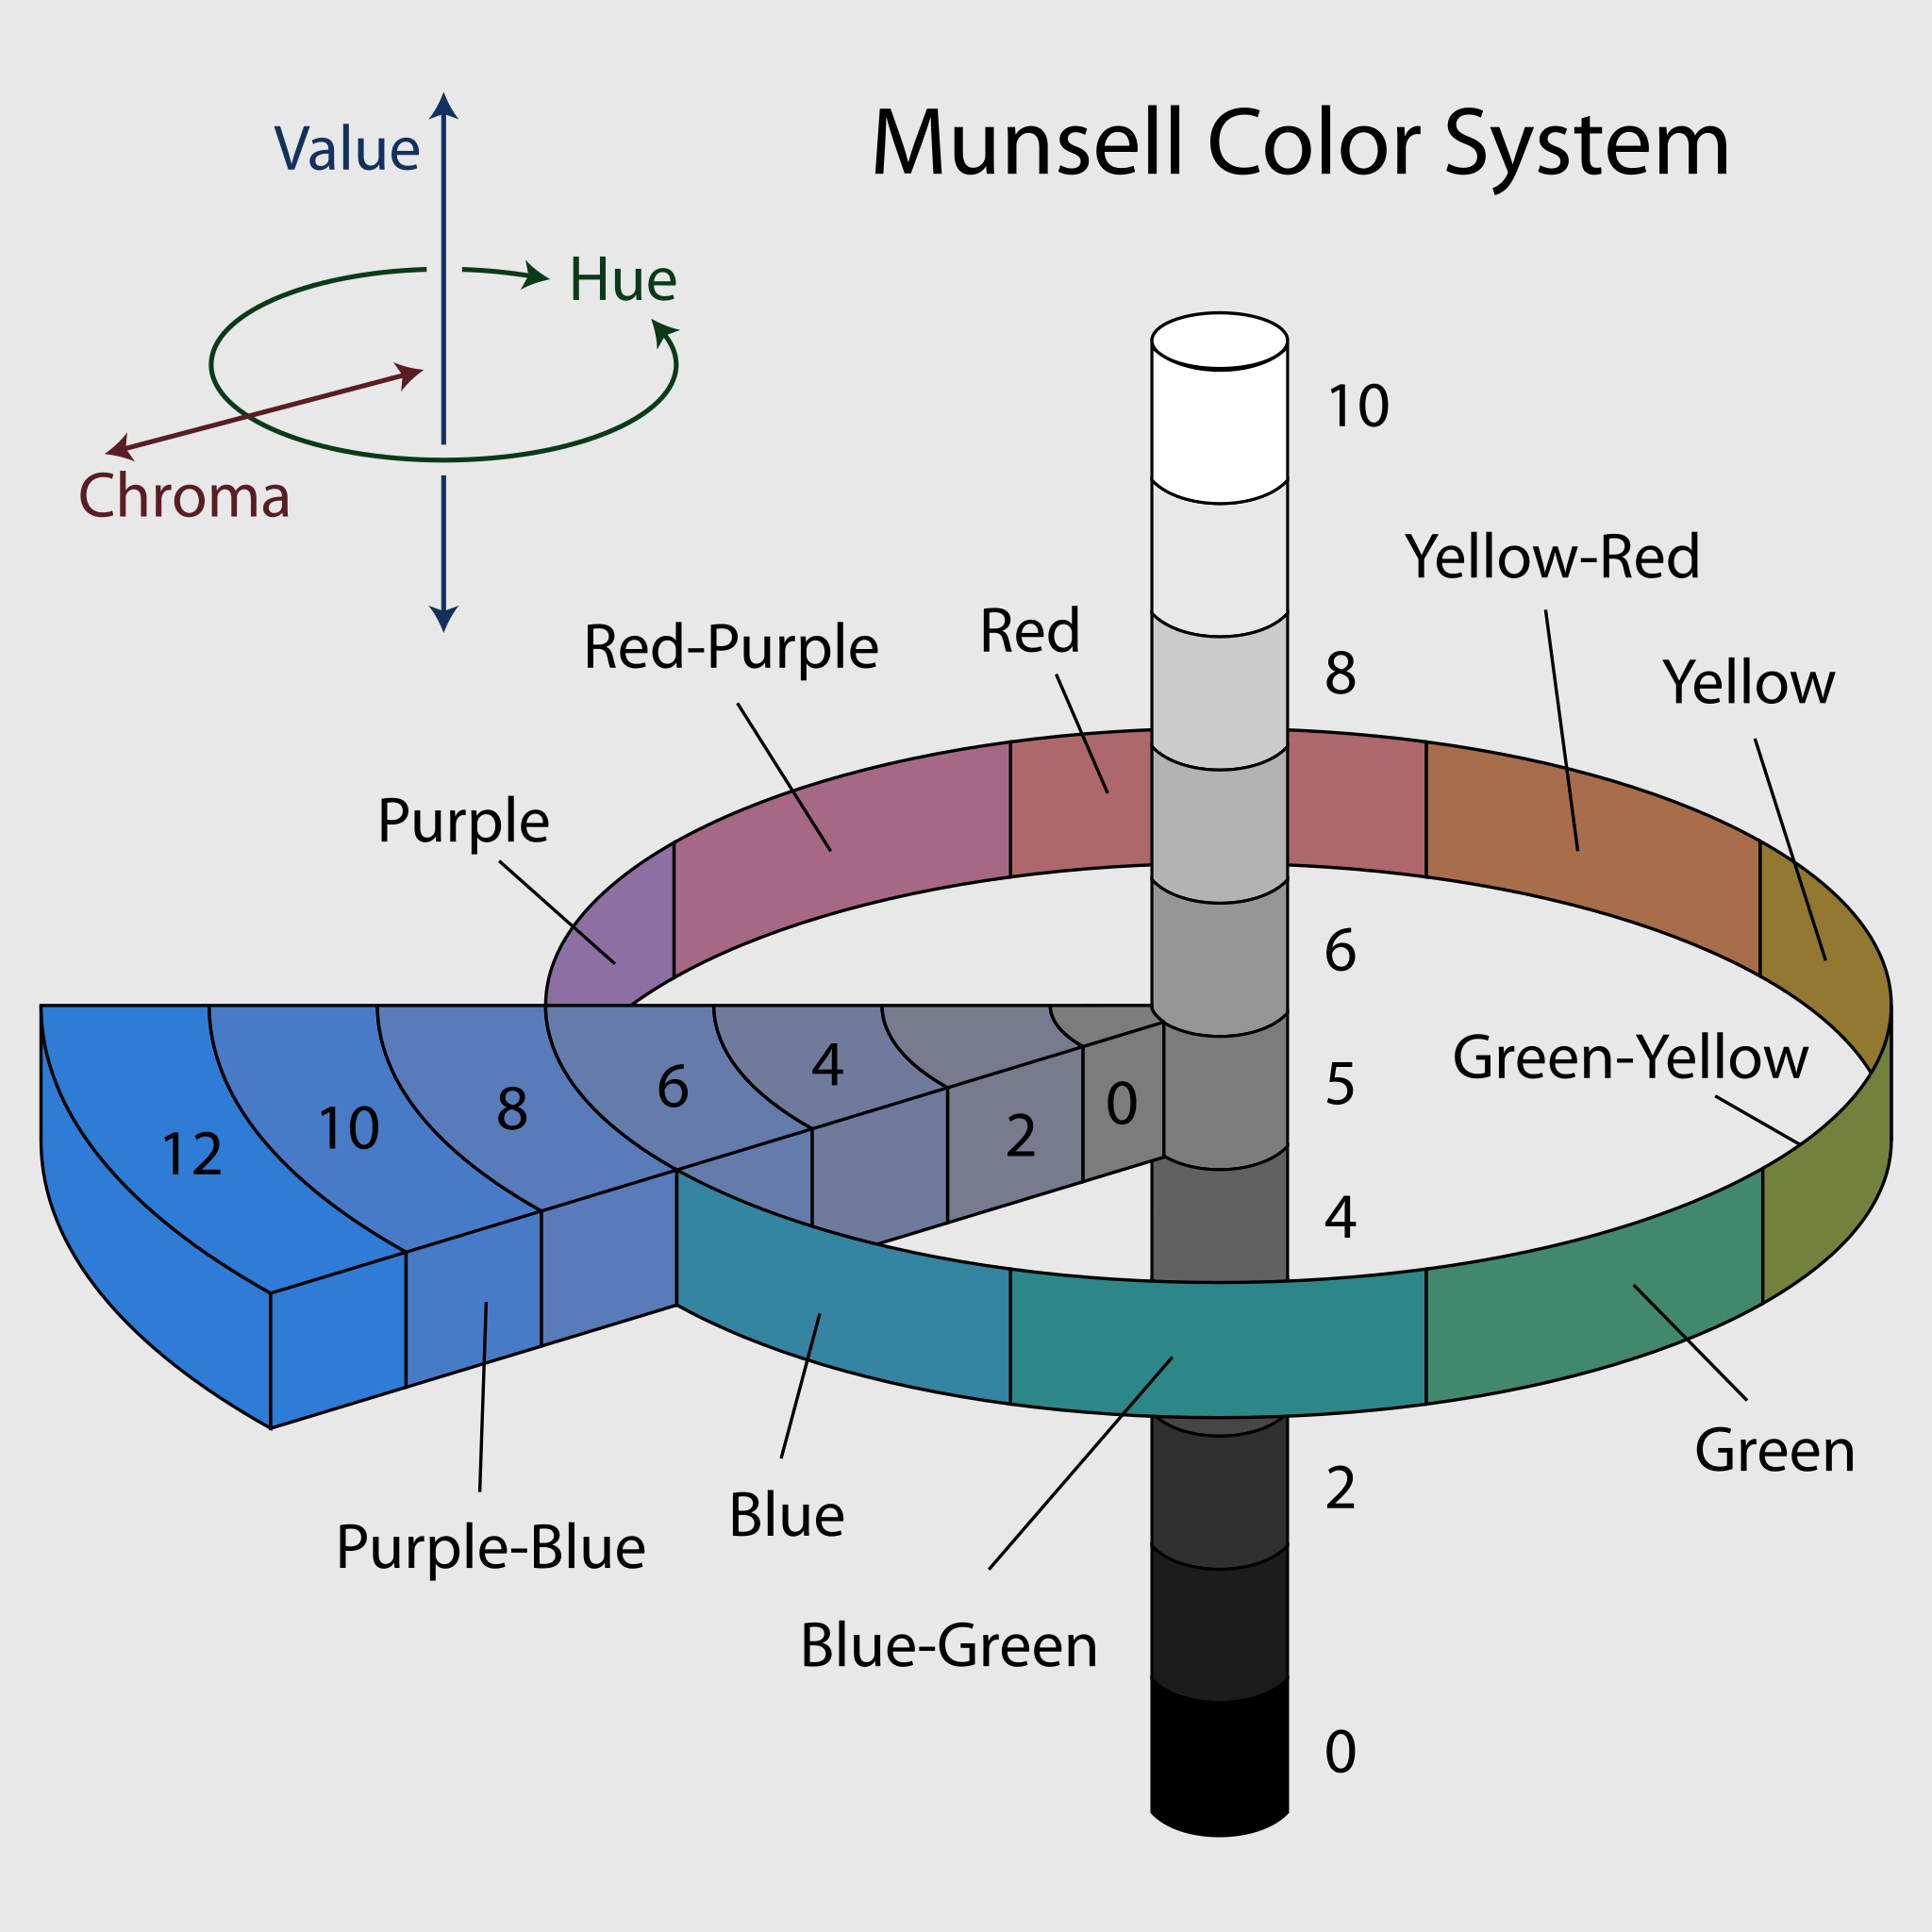
\includegraphics[width=1.0\columnwidth]{images/2048px-Munsell-system.svg.png}
    \includesvg[width=0.75\columnwidth]{Munsell-system.svg}
    \caption{A diagram of the Munsell Color System. The image shows i) the neutral values in steps of 1 from 0 to 10 in a vertical orientation ii) a circle of 10 hues at value 5 and chroma 6, and iii) the chromas of purple-blue in steps of 2 from 0 to 12, at value 5. From Rus 2007 Creative Commons Attribution-Share Alike 3.0 Unported.}
    \label{fig:MunsellColorSystem}
\end{figure}

Previously the example given was 10YR 5/4 where 10YR is the hue, 5 is the value, and 4 is the chroma.

This section on color started by stating that there are 'inferences' derived from color. Actually, it is slightly more interesting because it is not just the determination of color but also the distribution of differences in color in the soil  within or on the surface of a ped or other voids.

One technical classification is very dependent upon the morphology of soil color and in particular redox. The reduction of iron and manganese under reducing conditions, such as saturation with water in warm conditions, results in them being  transported (are more mobile when reduced) and reoxidized when the water drains. These patterns of depleted areas interspersed with areas displaying oxidized iron (rubified) and manganese (brown colored) indicate, or are interpreted as, arising from a fluctuating water table. The depth at which these redoximorphic features occur together with the timing and length of saturation leads to \textbf{drainage class}.

\begin{tcolorbox}[enhanced, attach boxed title to top center={yshift=-3mm, yshifttext=-1mm}, colback=yellow!18!white, colframe= red!55!black, colbacktitle=red!65!black, title=redoximorphic features, fonttitle=\bfseries, boxed title style={size=small, colframe=red!50!black} ]
Features formed by the processes of reduction, translocation, and/or oxidation of Fe and Mn oxides; formerly called mottles and low-chroma colors. \end{tcolorbox}

\begin{tcolorbox}[enhanced, attach boxed title to top center={yshift=-3mm, yshifttext=-1mm}, colback=yellow!18!white, colframe= red!55!black, colbacktitle=red!65!black, title=Redox depletions, fonttitle=\bfseries, boxed title style={size=small, colframe=red!50!black} ]

Bodies of low chroma (2 or less) having value of 4 or more where Fe-Mn oxides have been stripped or where both Fe-Mn oxides and clay have been stripped. \textit{Redox depletions contrast distinctly or prominently with the matrix.}
\end{tcolorbox}

\begin{tcolorbox}[enhanced, attach boxed title to top center={yshift=-3mm, yshifttext=-1mm}, colback=yellow!18!white, colframe= red!55!black, colbacktitle=red!65!black, title=Reduced matrix, fonttitle=\bfseries, boxed title style={size=small, colframe=red!50!black} ]
A soil matrix that has low chroma and high value, but in which the color changes in hue or chroma when the soil is exposed to air.
\end{tcolorbox}

\begin{tcolorbox}[enhanced, attach boxed title to top center={yshift=-3mm, yshifttext=-1mm}, colback=yellow!18!white, colframe= red!55!black, colbacktitle=red!65!black, title=gleyed matrix, fonttitle=\bfseries, boxed title style={size=small, colframe=red!50!black} ]
Soils with a gleyed matrix have the following combinations of hue, value, and chroma (the soils are not glauconitic):
\begin{enumerate}
  \item A hue of 10Y, 5GY, 10GY, 10G, 5BG, 10BG, 5B, 10B, or 5PB with value of 4 or more and chroma of 1; or
  \item A hue of 5G with value of 4 or more and chroma of 1 or 2; or
  \item A hue of N with value of 4 or more; or
  \item In some places the gleyed matrix may change color upon exposure to air. This phenomenon is included in the concept of gleyed matrix.
\end{enumerate}
\end{tcolorbox}

\begin{tcolorbox}[enhanced, attach boxed title to top center={yshift=-3mm, yshifttext=-1mm}, colback=yellow!18!white, colframe= red!55!black, colbacktitle=red!65!black, title=Glauconitic,   fonttitle=\bfseries, boxed title style={size=small, colframe=red!50!black} ]
Refers to a mineral aggregate that contains a micaceous mineral resulting in a characteristic green color
\end{tcolorbox}
 
\subsection{Soil Drainage Classes}
\label{drainageclasses}

Soil drainage class is a way of communicating internal soil drainage conditions together with the depth in the soil that reducing conditions were, or are, as determined by soil redoximorphic features.

There are seven such classes. The soil is examined to a depth of \qty{150}{cm}.

\textbf{Excessively drained}: Water is removed very rapidly (gravelly or coarse sand textures). The occurrence of free water is very deep (\textgreater{}\qty{150}{cm} or 60\,in). Free of redoximorphic features related to wetness.

\textbf{Somewhat excessively drained}: Water is removed from the soil rapidly (sands and loamy sand textures). The occurrence of free water commonly is very deep (\textgreater{}\qty{150}{cm} or 60\,in). Free of redoximorphic features related to wetness.

\textbf{Well drained}: Water it removed readily but not rapidly. Free water occurrence is deep (\textgreater{}\qty{150}{cm} or 60\,in). Well drained soils are generally free of redoximorphic features related to wetness in the upper \qty{150}{cm} (or 60\,in). There may be mottles deeper in the soil profile.

\textbf{Moderately well drained}: Water is removed from the soil somewhat slowly during some periods of the year. Free water occurrence is moderately deep (\qtyrange{50}{100}{cm}) and transitory (\numrange{1}{3} months) to permanent (continuous). The soils are wet for only a short time within the rooting depth during the growing season. Moderately well drained soils may have redoximorphic features below a depth of \qty{50}{cm} (about\,20 in.). It is common for moderately well drained soils to have a slowly permeable layer within or immediately beneath the solum or a relatively high water table.

\textbf{\textit{Somewhat poorly drained}}: Water is removed slowly so that the soil is wet at a shallow depth for significant periods during the growing season. The occurrence of free water is shallow (\qtyrange{25}{50}{cm} or 10 to 20\,in.) and transitory (1 to 3 months) or common (present 3 to 6 months). Wetness markedly restricts the growth of many common crop plants unless artificial drainage is provided. They commonly have a high water table, and redoximorphic features occur below a depth of \qty{25}{cm} (about 10\,in.). These soils often have thick dark A horizons high in organic matter.

\textbf{Poorly drained}: Water is removed so slowly that the soil is wet at shallow depths periodically during the growing season or remains wet for long periods. The occurrence of free water is shallow or very shallow (\textless{}\qty{25}{cm} about 10 in.) and common (\numrange{3}{6} months) or persistent (6 through 12 months). Free water is commonly at or near the surface long enough during the growing season so that mesophytic crops cannot be grown without artificial drainage. These soils are commonly gleyed rather than redoximorphic  because they remain anoxic for long periods.

\textbf{Very poorly drained}: Water is removed from the soil so slowly that free water remains at or very near the ground surface during much of the growing season. The occurrence of free water is very shallow and persistent or permanent.

\section{Consistence}
\label{consistence}

Soil consistence is dependent upon moisture content and consequently is measured and reported at three moisture statuses: dry, moist, and wet. For the engineering learner it is important to note that the tests of soil consistence differ from consistency. The tests applied to determine soil consistence are derived principally as being those could be applied in a field setting.

Principal to the outcome of soil consistence classes reported for soil is the soil cohesion and adhesion and resistance to deformation and/or rupture. The classes include rupture resistance class, plasticity class, toughness class, and stickiness class.

\textbf{Rupture Resistance} classes for moist soils span from cohesion-less soils that include the coarser texture classes of sand and loamy sand that are \textit{loose} and progress though successively greater force being applied to a moist ped or clod. These field tests begin with determination of failure when a quantitative force is applied between thumb and forefinger–\textit{very friable}, to \textit{friable}, to \textit{firm}, to \textit{very firm}–progresses to force applied between hands (\textit{extremely firm}), to force exerted underfoot (\textit{rigid}), and finally to the force being a blow caused by a \qty{2}{kg} weight being dropped from a height of \qty{15}{cm} (\textit{very rigid}). In addition to the presented classes above that are determined on moist soil their exists  collections of descriptive terms for rupture resistance of dry peds or clods and for those with cementation.

\textbf{Plasticity Class} is determined on \enquote{puddled} soil at the water content that yields the maximum plasticity. Thus plasticity is the degree of permanent deformation the soil can exhibit without rupturing. Soil is formed into rolls \qty{4}{cm} long and \qty{6}{cm}, \qty{4}{cm}, or \qty{2}{cm} in diameter. The classes are \textit{nonplastic}, \textit{slightly plastic}, \textit{moderately plastic}, or \textit{very plastic}.

\textbf{Toughness Class}, \textit{low},  \textit{medium}, or \textit{high} based on the force necessary to form a \qty{3}{milli\metre} roll with the fingers.

\textbf{Stickiness Class} is, not surprisingly, categorizing soil ability to adhere to other objects. Similar to the plasticity and toughness classes determinations the determination is made on the water content at which the soil is most sticky. The four classes are \textit{nonsticky}, \textit{slightly sticky}, \textit{moderately sticky}, and \textit{very sticky}.

 % dig-soilman: A possible add-on as an appendix or supplement would be definitions for each of the consistence classes. Not sure about them being presented as a definition list or tabular greater than that presented above in the section itself. This would not be necessary to learners at all institutions, but some might find the inclusion helpful.
 
\section{Reaction}
\label{reaction}

Soil reaction is a way of communicating soil pH. Today it is generally inadvisable to place soil in the mouth, but the human palate is quite adept at determine various levels of sourness–increased acidity–and chalkiness–increased alkalinity. The pH today can be readily measured digitally with inexpensive handheld meters. The soil reaction classes pH ranges are presented in Table \ref{tab:reactionclass}. See a treatise on soil chemistry for more. % Altering this last sentence to a treatise on "Soil Chemistry" and should have reference if the two are bound.

\begin{table}[!htbp]
\centering
\caption{Table of soil reaction class terms and the corresponding ranges in pH.}
\label{tab:reactionclass}
\begin{tabular}{ll}
\hline
Class term             & pH range         \\ \hhline{==}
Ultra acid             & \textless 3.5    \\
Extremely acid         & 3.5–4.4          \\
Very strongly acid     & 4.5–5.0          \\
Strongly acid          & 5.1–5.5          \\
Moderately acid        & 5.6–6.0          \\
Slightly acid          & 6.1–6.5          \\
Neutral                & 6.6–7.3          \\
Slightly alkaline      & 7.4–7.8          \\
Moderately alkaline    & 7.9–8.4          \\
Strongly alkaline      & 8.5–9.0          \\
Very strongly alkaline & \textgreater 9.0 \\
\hline
\end{tabular}
\end{table}

% dig-soilman:: Below is a markdown table format corresponding to the above LaTeX table.
% Table of soil reaction class terms and the corresponding ranges in pH.
% | Class term             | pH range |
% |------------------------|----------|
% | Ultra acid             |  < 3.5   |
% | Extremely acid         | 3.5–4.4  |
% | Very strongly acid     | 4.5–5.0  |
% | Strongly acid          | 5.1–5.5  |
% | Moderately acid        | 5.6–6.0  |
% | Slightly acid          | 6.1–6.5  |
% | Neutral                | 6.6–7.3  |
% | Slightly alkaline      | 7.4–7.8  |
% | Moderately alkaline    | 7.9–8.4  |
% | Strongly alkaline      | 8.5–9.0  |
% | Very strongly alkaline |  > 9.0   |

% dig-soilman:: Reaction section is to be populated by an ever-so-brief description of reaction as historically discernible as sour versus chalky when placed in the mouth. Today placing soil in ones mouth is generally discouraged and there are relatively inexpensive ways to determine reaction class that are also more amenable to placing the soil in more classes that have more interpretive meaning. 
 
 
 \section{Effervescence}
 \label{effervescence}
 
% dig-soilman:: How to determine while describing a soil and the classes  presented in in succinct fashion.

A common description in soils of simiarid and arid landscapes is that of \textit{effervescence}. Carbonates of divalent cations, primarily calcium carbonate, effervesce when 1-normal hydrochloric acid (1N HCl) is applied. The relative strength of effervescence is classed and the classes and criteria are presented in Table \ref{tab:effervescenceclasses}.

Calcium carbonate content can increase alkalinity, increase color value, and even become cemented. 

If the surface of the soil is noneffervescent and the soils parent material is not carbonaceous, e.g. limestone or dolomite, then the depth at which the soil exhibits effervescence is likely largely influence by the effective precipitation owing to inadequate percolation to transport the carbonates below the soil profile, leaching. If carbonates are not removed from the soil profile than salts may also not be removed.

Salts are have greater solubility than carbonates so the appearance of carbonates does not necessitate an accumulation of salts. Salts can also increase color value and increase alkalinity, but have quite different implications for soil use and salts are not so easily distinguished in a field setting so chemical laboratory procedures are employed if called for. See a treatise on soil chemistry for more. % Altering this last sentence to a treatise on "Soil Chemistry" and should have reference if the two are bound.

Salts and carbonates can feed back to color and when their contents increase significantly results in greater Munsell values and chromas.

The effervescence class is only semi-quantitative. Laboratory methods exist to refine and determine carbonate equivalence and carbon content.

\begin{table}[!htbp]
\centering
\caption{Table of Effervescence Classes and Criteria.}
\label{tab:effervescenceclasses}
\begin{tabular}{ll}
\hline
Effervescence Class         & Criteria                          \\ \hhline{==}
Noneffervescent             & No Bubbles form                   \\
Very slightly effervescent  & Few bubbles form                  \\
Slightly effervescent       & Numerous bubbles foam             \\
Strongly effervescent       & Bubbles form a low foam           \\
Violently effervescent      & Bubbles quickly form a thick foam \\
\hline
\end{tabular}
\end{table}

% dig-soilman:: Below is a markdown table format corresponding to the above LaTeX table.
% Table of Effervescence Classes and Criteria
% | Effervescence Class        | Criteria                          |
% |----------------------------|-----------------------------------|
% | Noneffervescent            | No Bubbles form                   |
% | Very slightly effervescent | Few bubbles form                  |
% | Slightly effervescent      | Numerous bubbles foam             |
% | Strongly effervescent      | Bubbles form a low foam           |
% | Violently effervescent     | Bubbles quickly form a thick foam |

% dig-soilman:: ToDo Example study questions construction is a potential
% 	add-on. The down side is that as of 2022 the propensity for the
% 	solutions to such questions on study boards negates there
% 	effectiveness. Consequently dig-soilman favors NOT adding study
% 	questions directly to the end of the document and instead expects
% 	instructors leveraging the document to create there own.

\newpage
\quad % without \quad no new page would be inserted!!!
\newpage

\section*{Bibliography} % no BibTeX so access to the file provides ready access to the few items as opposed having to access another file

\begin{thebibliography}{}

    \bibitem{Bouyoucos1962}
    Bouyoucos, G. J., 1962. Hydrometer method improved for making particle size analysis of soils. Agron. J. 54:464-465.
    
    \bibitem{Rus20007}
    Rus, J. 2007. The Munsell color system. Creative Commons Attribution ShareAlike3.0 license \href{https://commons.wikimedia.org/wiki/File:Munsell-system.svg}{https://commons.wikimedia.org/wiki/File:Munsell-system.svg}

    \bibitem{SSS1999}
    Soil Survey Staff. 1999. Soil taxonomy: A basic system of soil classification for making and interpreting soil surveys. 2nd edition. Natural Resources Conservation Service. U.S. Department of Agriculture \href{./https://www.nrcs.usda.gov/Internet/FSE_DOCUMENTS/nrcs142p2_051232.pdf}{Handbook 436}.

    \bibitem{SSS2012}
    Soil Survey Staff. 2012. Field Book for Describing and Sampling Soils version 3.  USDA Natural Resources Conservation Services. \href{./https://www.nrcs.usda.gov/Internet/FSE_DOCUMENTS/nrcs142p2_052523.pdf}{Online version}

    \bibitem{SSS2014}
    Soil Survey Staff. 2014. Keys to soil taxonomy, 12th edition. USDA Natural Resources Conservation Services, Washington, DC. \href{https://www.nrcs.usda.gov/wps/portal/nrcs/detail/soils/survey/class/?cid=nrcs142p2_053580}{Online portal}

    \bibitem{SSS2017}
    Soil Survey Staff. 2017. Soil survey manual. C. Ditzler, K. Scheffe, and H. C. Monger (eds). USDA Handbook 18. Government Printing Office, Washington, D.C. \href{https://www.nrcs.usda.gov/wps/portal/nrcs/detail/soils/ref/?cid=nrcs142p2_054262}{Online portal}

    \bibitem{Thein1979}
    Thein, S. J. 1979. A flow diagram for teaching texture-by-feel analysis. J. Agron. Edu. 8:54-55. \href{https://doi.org/10.2134/jae.1979.0054}{https://doi.org/10.2134/jae.1979.0054}

    \bibitem{USDA-NRCS2018}
    United States Department of Agriculture, Natural Resources Conservation Service. 2018. Field Indicators of Hydric Soils in the United States, Version 8.2. L.M. Vasilas, G.W. Hurt, and J.F. Berkowitz (eds.). USDA, NRCS, in cooperation with the National Technical Committee for Hydric Soils. \href{https://www.nrcs.usda.gov/wps/portal/nrcs/main/soils/use/hydric/}{Online portal}
\end{thebibliography}


\end{document}